% =====================================================================
% ASKING CLAUDE FOR SOMETHING IN THIS PAPER
%
% Write your request as a LaTeX comment, in the TEXT, on the line above
% the passage it is about, and sign it:
%
%     % [CLAUDE/GB: is the 12 h window defensible, or should it be 24?]
%
% Claude answers in place, leaving both lines for you to find:
%
%     % [CLAUDE-REPLY: crest times are bimodal (h29-42, h60-72) with an
%     %  empty gap, so 24 h integrates marks that already peaked. Kept.]
%
% Delete the pair once you are satisfied.
%
% Three things to know:
%
%   1. Overleaf MARGIN COMMENTS DO NOT REACH CLAUDE. They are stored
%      outside the document and never appear in the git history Claude
%      reads. A request left in a comment thread will not be seen.
%      Use the code editor, not the visual editor, which hides % lines.
%
%   2. Nothing notifies Claude. Mark triggers the read, so expect the
%      latency to be "next working session", not minutes.
%
%   3. Claude acts directly on editorial requests -- wording, structure,
%      notation, citations, captions. Anything that would change a
%      NUMBER, a SCIENTIFIC CLAIM, an attribution, or the author list is
%      routed to Mark instead of executed: those come from runs, and a
%      comment cannot change what a run produced.
%
% Sign your marker. The answer often depends on who is asking.
% =====================================================================

\documentclass[11pt]{article}
\usepackage[margin=1in]{geometry}
\usepackage{amsmath}
\usepackage{amssymb}
\usepackage[hidelinks]{hyperref}
\usepackage{booktabs}
\usepackage{graphicx}
\usepackage{xcolor}
\usepackage{algorithm}
\usepackage{algpseudocode}
\usepackage{pgfplots}
\pgfplotsset{compat=1.18}

\title{Adjoint measurement and calibration of Manning roughness in
E3SM's river dynamical core\\[4pt]\large DRAFT for internal review}
\author{Mark Adams$^1$, Gautam Bisht$^2$, Donghui Xu$^2$, Jeffrey
Johnson$^3$, Jed Brown$^4$, Matthew Knepley$^5$\\[2pt]
\footnotesize $^1$Applied Mathematics \& Computational Research Division,
Lawrence Berkeley National Laboratory, Berkeley, CA, USA\\
\footnotesize $^2$Atmospheric, Climate, \& Earth Sciences Division, Pacific
Northwest National Laboratory, Richland, WA, USA\\
\footnotesize $^3$Cohere Consulting, LLC, Seattle, WA, USA\\
\footnotesize $^4$Department of Computer Science, University of Colorado
Boulder, Boulder, CO, USA\\
\footnotesize $^5$Computer Science and Engineering, University at Buffalo,
Buffalo, NY, USA}
\date{}

\begin{document}
\maketitle

\begin{abstract}
This paper presents a transient discrete adjoint of RDycore, the river
dynamical core of the Energy Exascale Earth System Model (E3SM), and
uses it to measure how much of a flood model's error its roughness
parameter is able to remove. We differentiate the production solver in
place rather than rewrite it in a differentiable-programming
framework: one exact, assembled Jacobian of the shallow-water
right-hand side serves the implicit time integrator, the adjoint, and
the calibration. An objective and its gradient cost about two forward
solves regardless of the number of parameters, every derivative passes
a finite-difference gate on the full nonlinear solve, and the whole
gradient path runs on GPUs, where four NVIDIA A100s run a calibration
iteration on a dense-gauge twin $19\times$ faster than a 64-core CPU
node.

For Hurricane Harvey on a 2.93M-cell, 30\,m mesh of the Houston area,
scored against 46 surveyed high-water marks, the ceiling of Manning
roughness is measurable before any optimizer runs. A single factor on
the whole roughness field removes at most $0.08$\,m of a $0.72$\,m
error, and only at roughness values below any entry in the lookup;
fifteen land-cover classes calibrated separately remove $0.107$\,m,
$15\%$ of the error. The spectrum of the prior-preconditioned
Gauss--Newton Hessian, from sixteen forward runs, shows why: at a
$\pm 30\%$ width on the land-cover lookup, the marks determine about
three combinations of the fifteen classes, and calibrating those three
recovers $84\%$ of what fifteen achieve. What the three reach is the
same at every prior width we ran: developed-medium and woody wetland
at $0.3\times$ their lookup values, below the lookup's value for
developed open land. The calibrated friction is compensating for an
error that is not in the friction.
What a $\pm 30\%$ prior cannot support is the fifteen-class field. The
survey is the observable because at seven of twelve stream gauges the
30\,m cell's bed sits above the peak observed water surface: the mesh
holds the bank of an incised bayou, not its channel. Calibrating the
same three classes on the gauges that do hold water sends them the
opposite way, to the top of the prior instead of the bottom, and the
resulting field scores worse at the marks than no calibration at all.
Roughness is absorbing each observable's own error.
Pointed at the initial state, the same measurement finds more: a
$20\%$ reduction in stored water is worth $0.075$\,m. Most of the
remaining error lives in the model's water balance, not in its
friction.
\end{abstract}

\section{Introduction}

Manning roughness is the dominant tunable parameter of depth-averaged
flood models, and its calibration is traditionally manual or ensemble
based. Adjoint methods deliver the gradient of an observation misfit
with respect to \emph{every} cell's roughness at a cost that does not
grow with the number of parameters --- a few forward solves, measured
in Section~\ref{sec:calibration} --- making distributed calibration
tractable. The
approach is well established in shallow-water modeling, from channel
networks~\cite{ding2004manning} and unstructured finite-volume
\emph{twin experiments} --- calibrations against observations the
model itself generated from a known roughness field, so that the
recovered field can be scored against a truth, and unrelated to the
``digital twin'' of a physical asset~\cite{yan2014adjoint} --- to
GPU-accelerated
optimizers~\cite{lacasta2016gpu}. It is deployed in
variational-assimilation platforms such as
DassFlow~\cite{dassflow,lai2009assimilation,brisset2018swot} and the
Thetis coastal model,
which calibrated a spatially varying Manning field for the Baltic Sea
with an automatically generated adjoint~\cite{karna2023baltic},
following storm-surge sensitivity studies that addressed the
overfitting inherent in distributed friction
estimation~\cite{warder2021storm}. The closest published work to ours
is Pujol et al.~\cite{pujol2024urban}, who infer distributed friction in
a 2D urban flood model by variational assimilation of multi-source data
\emph{including high-water marks}, and use adjoint-derived global
sensitivity measures to decide how to spatialize the friction field
before assimilating --- the same observable and the same design move
that Sections~\ref{sec:hwm} and~\ref{sec:authority} employ, at street
scale and with a Tapenade-generated adjoint of a solver built for
assimilation. What this paper adds is neither the adjoint nor the
observable but the setting and the question: a production Earth-system
component differentiated in place, and a measurement of how much of
the model's error the parameter can explain at all. For this event and
this observable the answer is $15\%$, and the spectrum of the
calibration problem explains it: the marks determine about three
roughness combinations, so a calibration of three parameters recovers
most of what fifteen achieve and a wide prior releases the twelve it
cannot determine. The measurement is not specific to roughness, and
Section~\ref{sec:icauthority} turns it on the model's initial state,
where it finds more.

A recent generation of \emph{differentiable} flood and hydrology codes
obtains gradients by rewriting simplified solvers inside
machine-learning frameworks: Inunda (PyTorch, local-inertial, calibrated on a Hurricane
Harvey hindcast)~\cite{li2026inunda}, Hydrograd
(Julia)~\cite{liu2025uswe}, AegirJAX~\cite{cardoso2026aegir}, and
differentiable routing~\cite{bindas2024routing}. These demonstrate
demand for exactly this capability, but none is a production
Earth-system component: they trade the validated numerics, unstructured
meshes, and coupling infrastructure of codes like RDycore for
differentiability. A parallel line ports production hydrodynamics to
GPUs without differentiating them --- CaMa-Flood-GPU~\cite{kang2026cama}
is a GPU reimplementation of CaMa-Flood, with gradient-based
calibration named as future work rather than demonstrated.

This paper takes the complementary route: make the production code
differentiable. That route has a long precedent outside E3SM --- most
prominently MITgcm, whose exact adjoint is generated by automatic
differentiation of the production ocean model~\cite{heimbach2005mitgcm}
and underpins two decades of ECCO state and parameter
estimation~\cite{forget2015ecco}. Ours differs in how the derivative is
obtained rather than in ambition: the Jacobian is hand-differentiated
and assembled, which makes it available to the implicit solver as well
as to the adjoint, and Section~\ref{sec:implicit} argues that for a
differentiable friction term the implicit solve is not optional. Inside
E3SM the precedent is narrower: the
land-ice component MALI~\cite{hoffman2018mali} routinely inverts for
basal friction with an adjoint obtained by automatic differentiation of
its Albany velocity solver~\cite{perego2014initialization} --- but that
is the adjoint of a \emph{steady} nonlinear solve, used for
initialization; no E3SM component has, to our knowledge, a discrete
adjoint of its transient time stepper. RDycore is a finite-volume
shallow-water dynamical core
(Roe fluxes, well balancing, wetting and drying) validated at up to 471M
cells. We add the missing derivative infrastructure --- an exact
assembled Jacobian and TSAdjoint-based sensitivities
\cite{zhang2022tsadjoint} --- entirely behind a configuration flag, with
no impact on existing runs and no new dependencies.

This paper contributes:
\begin{itemize}
  \item an exact Jacobian of the shallow-water right-hand side ---
        Roe dissipation, entropy-fix and wet/dry branches, and
        reflecting, Dirichlet and critical-outflow boundaries ---
        verified against finite differences to $10^{-6}$
        (Section~\ref{sec:jacobian});
  \item adjoint gradients with respect to the initial state and the
        roughness field, at multiple observation times, verified to
        $10^{-5}$ or better (Section~\ref{sec:adjoint});
  \item implicit backward-Euler stepping and its adjoint from the same
        Jacobian, with the measurement that the explicit friction term
        returns a non-finite state at every step tested on the 30\,m
        Hurricane Harvey mesh (Section~\ref{sec:implicit});
  \item a measurement of when an observing network makes a roughness
        field identifiable at all, from twin experiments and from the
        spectrum of the prior-preconditioned Gauss--Newton Hessian,
        which counts the roughness combinations the observations
        determine (Sections~\ref{sec:houston} and~\ref{sec:spectrum});
  \item the ceiling of roughness on the Hurricane Harvey survey error,
        $15\%$, and the three-parameter calibration the spectrum
        selects (Sections~\ref{sec:authority}--\ref{sec:spectrum});
  \item a cross-observable validation: the three classes calibrated on
        the stream gauges move to the opposite edge of the same prior
        and score worse at the high-water marks than the uncalibrated
        lookup, which makes the survey-only result a fit rather than a
        skill (Section~\ref{sec:hwm});
  \item the same measurement applied to the initial state, where it
        finds more, and the diagnosis of the downstream reach as a
        ponded lake behind the domain's outlet
        (Sections~\ref{sec:hwm} and~\ref{sec:icauthority}).
\end{itemize}

\section{Methods}
\label{sec:methods}

\subsection{Forward model}
\label{sec:forward}

RDycore solves the 2D shallow water equations in conservative variables
$u = (h, q_x, q_y)$, $\mathbf{q} = h\mathbf{v}$:
\begin{align}
  \partial_t h + \nabla\!\cdot\!\mathbf{q} &= Q_r(x,t),\\
  \partial_t \mathbf{q}
    + \nabla\!\cdot\!\Big(\tfrac{\mathbf{q}\otimes\mathbf{q}}{h}
    + \tfrac{g h^2}{2}\,\mathbb{I}\Big)
  &= -\,g h \nabla z_b \;-\; g\, n^2 h^{-7/3}\,\mathbf{q}\,\lVert\mathbf{q}\rVert,
  \label{eq:mom}
\end{align}
with cell-centered finite volumes on an unstructured mesh:
\begin{equation}
  \frac{du_i}{dt}
  = -\frac{1}{|\Omega_i|}\sum_{e \in \partial\Omega_i}
      \mathcal{F}\big(u_i, u_j, \mathbf{n}_e\big)\,L_e + S(u_i; n_i, t)
  \equiv f_i(u, n),
  \label{eq:semidiscrete}
\end{equation}
where $\mathcal{F}$ is the Roe flux with a critical-flow (entropy) fix,
primitives are reconstructed with a regularized division and a dry
cutoff $h_{\min}$, and $S$ contains bed slope, Manning drag, and
external forcing.

The Roe flux's dissipation is built from the moduli $|\lambda_p|$ of
its characteristic wave speeds, so the closed-form expression it
evaluates switches wherever a wave speed changes sign. Switches like
this, \emph{branches} in the sense that $|x|$ has a positive and a
negative branch, recur throughout the discretization. They belong to
the model rather than to the derivative: a nonlinear solver must
accommodate them whether or not anyone differentiates the code, which
is the argument of Section~\ref{sec:implicit}.
Away from a switching surface the map is smooth and equals its active
branch; the derivative machinery of
Sections~\ref{sec:jacobian}--\ref{sec:adjoint} is
\emph{branch-faithful}, differentiating the expression the condition
actually selected to give the correct one-sided derivative.

\paragraph{A differentiable right-hand side.}
RDycore's existing friction treatments (a semi-implicit splitting and
the implicit scheme of Xia and Liang) embed the time step, and in the
semi-implicit case the flux divergence, inside the RHS callback. The
resulting map is consistent only with forward Euler and admits no
well-defined $\partial f/\partial u$. We therefore added a plain
explicit source treatment (\texttt{source.method: explicit}), used on
every adjoint path, and Section~\ref{sec:implicit} shows how the
implicit integrator, rather than the right-hand side $f$, then handles
the resulting stiffness.

\subsection{Differentiating the production solver}
\label{sec:diff}

Two design decisions shape everything downstream. We obtain the
derivative of the right-hand side by hand, as forward-mode
differentiation of the flux computation itself, branch by branch, and
we \emph{assemble} it into a sparse matrix rather than apply it
matrix-free. Assembly is what lets one artifact serve three consumers:
the implicit solver preconditions with it
(Section~\ref{sec:implicit}), \texttt{TSAdjoint} transposes it, and
the calibration couples it to the parameter Jacobian. The two parts
below build that Jacobian (Section~\ref{sec:jacobian}) and the adjoint
sensitivities on top of it (Section~\ref{sec:adjoint}); every
derivative is gated by finite differences of the full nonlinear solve.

\subsubsection{Exact Jacobian}
\label{sec:jacobian}

The RHS Jacobian is block sparse with $3\times3$ blocks on the
cell-adjacency graph: each interior edge $(i,j)$ contributes
$\mp(L_e/|\Omega_{i,j}|)\,\partial\mathcal{F}/\partial u_{L,R}$ to the
two cell rows, local sources contribute diagonal blocks, and boundary
edges contribute diagonal blocks through the ghost-state map of the
boundary condition.

Edge orientation is a classical source of sign errors in this
construction, so one consequence of that structure needs stating. The
pair
$(\partial\mathcal{F}/\partial u_L, \partial\mathcal{F}/\partial u_R)$
is evaluated \emph{once} per edge, in the edge's own stored normal
direction, and then scattered to both cell rows with opposite area
weights $-L_e/|\Omega_i|$ and $+L_e/|\Omega_j|$: the downwind cell
receives the same two blocks with the roles of $u_L$ and $u_R$
exchanged between diagonal and off-diagonal positions. The normal is
never flipped and the flux routine is never re-entered with reversed
arguments, so conservation is structural rather than something the
signs must reproduce, mirroring how the right-hand side itself
accumulates the flux. The assembled-matrix
checks in Table~\ref{tab:verification} would expose any lapse
regardless, since they compare the full assembly against a
matrix-coloring finite-difference Jacobian of the actual RHS on
unstructured meshes with mixed boundary conditions, where a single
mis-oriented edge is visible.

\paragraph{Flux blocks by forward-mode differentiation.}
Rather than deriving the dissipation-matrix derivatives symbolically, we
differentiate the flux \emph{computation}: a hand-written forward-mode
(tangent) version of the Roe flux routine propagates directionals
through every intermediate (Roe averages, eigenvectors, eigenvalues
including both branches of the critical-flow fix, wave strengths, and
physical fluxes), taking the code's own branch at every $|\cdot|$ and
switch. The result is a consistent one-sided derivative. Seeding unit
directions through the primitive-reconstruction chain rule yields the
two conservative-space blocks in six tangent evaluations per edge. The
tangent code mirrors the flux code line by line, so it can be reviewed
against it, and we found it correct on first assembly against the
verification harness below.

\paragraph{Boundary blocks.}
For a boundary edge, $F(u_{\mathrm{in}}, u_g(u_{\mathrm{in}}))$
contributes $(\partial_L F + \partial_R F\, \partial u_g/\partial
u_{\mathrm{in}})$. The reflecting map is a linear mirror; Dirichlet
ghosts are constant; critical outflow has a closed-form ghost map
$h_g = (q^2/g)^{1/3}$ with the code's inflow branch producing an
identically zero flux.

\paragraph{Parameter Jacobian.}
Manning $n$ appears only in the drag term, so
$\partial S_{\mathbf q}/\partial n = -2 g n h^{-7/3}\mathbf{q}\lVert\mathbf q\rVert$:
two nonzeros per cell, supplied to \texttt{TSSetRHSJacobianP}.

\paragraph{Verification.}
Three layers, all against central finite differences, with the
pass/fail tolerances fixed in advance of the runs
(Table~\ref{tab:verification}): an edge-level
harness that differences the flux routine itself on sampled states (with
a Richardson self-check of the FD order); full-matrix comparisons of the
assembled Jacobian against a matrix-coloring FD Jacobian of the actual
RHS on three state/boundary combinations, boundary rows included; and
end-to-end gradient checks through the adjoint
(Section~\ref{sec:adjoint}). A
finite-difference coloring Jacobian (\texttt{numerics.jacobian: fd})
remains available permanently as the verification baseline.

\begin{table}
\centering\small
\begin{tabular}{@{}llll@{}}
\toprule
Check & Configuration & Result & Gate \\
\midrule
Edge flux blocks & wet jump $10\,\mathrm{m}/5\,\mathrm{m}$ & $7.6\times10^{-9}$ & $10^{-6}$ \\
Edge flux blocks & transcritical (entropy-fix branch) & $2.4\times10^{-10}$ & $10^{-5}$ \\
Source block & shallow flowing state & $<10^{-6}$ & $10^{-6}$ \\
Assembled matrix & uniform flow, reflecting BCs & $1.6\times10^{-8}$ & $10^{-6}$ \\
Assembled matrix & dam break, reflecting BCs & $1.5\times10^{-8}$ & $10^{-6}$ \\
Assembled matrix & dam break, Dirichlet + critical outflow & $1.9\times10^{-8}$ & $10^{-6}$ \\
$dJ/du_0$ (explicit RK) & 8 sampled components & $1.0\times10^{-8}$ & $10^{-5}$ \\
$dJ/dn$ (explicit RK) & domain aggregate & $2.9\times10^{-6}$ & $10^{-5}$ \\
$dJ/du_0$ (implicit BE) & tight inner tolerances & $1.4\times10^{-8}$ & $10^{-5}$ \\
$dJ/dn$ (implicit BE) & tight inner tolerances & $5.3\times10^{-6}$ & $10^{-5}$ \\
\bottomrule
\end{tabular}
\caption{Relative errors of analytic derivatives against central finite
differences of the full nonlinear computation. Every check in this
table is an automated test in RDycore's \texttt{ctest} suite, run on
every change to the repository.}
\label{tab:verification}
\end{table}

\subsubsection{Adjoint sensitivities}
\label{sec:adjoint}

For gauge observations $y_k$ at times $t_k$ with observation operator
$H$ (one row per gauge, selecting water height) and error variance
$\sigma^2$,
\begin{equation}
  J(n) = \tfrac{1}{2\sigma^2} \sum_k \lVert H u(t_k) - y_k\rVert^2 .
\end{equation}
\texttt{TSAdjoint}~\cite{zhang2022tsadjoint} differentiates the discrete
time stepper, so gradients are exact to roundoff for the computed
trajectory, which is the property that makes the FD gates in
Table~\ref{tab:verification} meaningful. Multi-time observations are
handled by a segmented backward sweep: the adjoint is advanced between
observation times with \texttt{TSAdjointSetSteps} and receives a jump
$H^T\sigma^{-2} r_k$ at each $t_k$
(Algorithm~\ref{alg:var4d} in Section~\ref{sec:calibration}). One sweep yields both $dJ/du_0$
(state sensitivity) and $dJ/dn$ (per-cell parameter gradient, via the
two-nonzero parameter Jacobian).

Two integrator facts constrain the design. PETSc's plain forward-Euler
integrator implements no adjoint, so adjoint-path configurations use the
Runge--Kutta family. And for implicit integrators the discrete-adjoint
gradient is only as exact as the inner solves: the Manning gradient
fails its gate at default inner tolerances and passes once they are
tightened (Table~\ref{tab:verification}, implicit rows). We found
loose inner tolerances a false economy on this problem: a tighter
Krylov tolerance makes the implicit forward \emph{faster}, because
better linear solves let Newton converge in fewer iterations, and the
production setting (Krylov $10^{-4}$, nonlinear $10^{-5}$) reproduces
the fully converged answer to every printed digit for about $25\%$
more wall time than the loosest usable setting. Campaigns therefore
run at converged inner tolerances, and the verified gradients
\emph{are} the production gradients. The FD gates cannot certify the
objective's own nonsmoothness over long windows, which
Section~\ref{sec:hwm} quantifies.

\subsection{The calibration algorithm: strong-constraint 4D-Var}
\label{sec:calibration}

The complete calibration loop is summarized in
Algorithms~\ref{alg:var4d}--\ref{alg:blmvm}. It is a strong-constraint
4D-Var iteration: the model is enforced exactly (the only controls are
the Manning field and, optionally, the initial state). Each objective
evaluation performs one checkpointed forward sweep that records the
gauge residuals $r_k$ at the observation times, followed by one
backward sweep of the discrete adjoint (Algorithm~\ref{alg:sweep}).
The per-iteration cost is therefore one forward sweep, the checkpoint
recomputation the backward sweep requires, and one adjoint sweep,
about $2.1$ forward solves in total at production settings
(Eq.~\eqref{eq:gradcost}) and independent of the number of parameters.
We measure that constant rather than assume it, since for a nonlinear
model on a memory-limited device the checkpointing scheme, not the
adjoint, sets it. Throughout, the
objective splits as $J = J_{\mathrm{mis}} + J_{\rm prior}$, where the
\emph{misfit} $J_{\mathrm{mis}} = (2\sigma^2)^{-1}\sum_k\lVert
r_k\rVert^2$ measures disagreement with the observations and
$J_{\rm prior}$ is the Tikhonov term of Eq.~\eqref{eq:sigman}. Only
$J_{\mathrm{mis}}$ needs the adjoint; the prior term's gradient is
closed form.

The backward sweep carries two vectors with distinct roles. The
\emph{adjoint state} $\lambda$ holds
$\partial J_{\mathrm{mis}}/\partial u(t)$ at the current point of the
backward traversal. It is seeded with the terminal observation
sensitivity $\sigma^{-2}H^T r_K$, propagated one step at a time by the
transposed Jacobian of the forward step map (the backward ``model
step''), and incremented by a jump $\sigma^{-2}H^T r_k$ each time the
sweep crosses an observation time, because the state at that time
enters the misfit directly. The \emph{parameter sensitivity} $\mu$
starts at zero and accumulates, at every step, the chain-rule
contribution $(\partial\Phi_s/\partial n)^T\lambda$ of that step's
Manning dependence. When the sweep reaches $t = 0$, $\mu$ is the
complete misfit gradient $dJ_{\mathrm{mis}}/dn$ and $\lambda$ is
$dJ_{\mathrm{mis}}/du_0$. Both transposed Jacobians are the analytic
operators of Sections~\ref{sec:jacobian}--\ref{sec:adjoint}, the
assembled RHS Jacobian for the state propagation and the two-nonzero
parameter Jacobian for the $\mu$ accumulation, applied within
\texttt{TSAdjoint}'s discrete adjoint of the chosen integrator.

The outer update is TAO's bound-constrained limited-memory
quasi-Newton method BLMVM~\cite{benson2001blmvm}
(Algorithm~\ref{alg:blmvm}). The loop terminates on the standard
bound-constrained test: the projected gradient $g^P$ (the gradient
with components pointing out of the feasible box zeroed) drops below
an absolute tolerance, or an iteration budget is reached. The
same loop serves every parameterization in this paper: per-region,
per-cell, and land-cover-class fields differ only in the expansion of
the parameter vector onto cells (line~\ref{ln:apply} of
Algorithm~\ref{alg:var4d}) and the corresponding summation of $\mu$
back onto parameters.

\begin{algorithm}
\caption{Strong-constraint 4D-Var calibration of the Manning field, as
implemented with TAO/BLMVM and \texttt{TSAdjoint}. The window map
$M_{t_{k-1}\to t_k}$ is the composition of $m$ steps of the discrete
forward stepper (explicit RK, backward Euler, or ARK-IMEX).}
\label{alg:var4d}
\begin{algorithmic}[1]
\Require prior/initial guess $n_0$, bounds $[n_{\min}, n_{\max}]$,
observations $y_k$ at times $t_k = k\,m\,\Delta t$ ($k = 1,\dots,K$),
gauge operator $H$, error $\sigma$, Tikhonov weight $\beta$, gradient
tolerance $\varepsilon_g$, iteration budget $I_{\max}$
\State $n \gets n_0$
\Repeat
  \State set the model's cellwise drag coefficient from $n$
         \label{ln:apply}
         \Comment{identity for per-cell $n$; constant over each region
         or land-cover class for the reduced parameterizations}
  \State $u \gets u_0$
         \Comment{fixed initial state (strong constraint)}
  \For{$k = 1, \dots, K$}
     \Comment{forward sweep; trajectory checkpointed --- every step, or
     a revolve schedule for long windows
     (Section~\ref{sec:implicit})}
     \State $u \gets M_{t_{k-1}\to t_k}(u;\, n)$
     \State $r_k \gets H u - y_k$
  \EndFor
  \State $J \gets \dfrac{1}{2\sigma^2}\sum_{k=1}^{K}\lVert r_k\rVert^2
          + \dfrac{\beta}{2}\lVert n - n_0\rVert^2$
  \State $(\lambda, \mu) \gets \Call{AdjointSweep}{\{r_k\}}$
         \Comment{Algorithm~\ref{alg:sweep} differentiates the stepper
         above, so $\mu = dJ_{\mathrm{mis}}/dn$ is exact to roundoff
         and inner-solver tolerance (Section~\ref{sec:adjoint})}
  \State $g \gets \mu + \beta\,(n - n_0)$
  \State $n \gets \Call{BlmvmStep}{n, J, g}$
         \Comment{Algorithm~\ref{alg:blmvm}}
\Until{$\lVert g^P \rVert \le \varepsilon_g$ or $I_{\max}$ iterations}
\State \Return $n$
\end{algorithmic}
\end{algorithm}

\begin{algorithm}
\caption{\textsc{AdjointSweep}: segmented discrete-adjoint backward
sweep (\texttt{TSAdjointSolve} with \texttt{TSAdjointSetSteps}).
$\Phi_s$ denotes the forward map of step $s$, $u_s =
\Phi_s(u_{s-1}; n)$; its transposed Jacobians are built from the
assembled RHS Jacobian $\partial f/\partial u$
(Section~\ref{sec:jacobian}) and the parameter Jacobian $\partial
f/\partial n$ according to the integrator's discrete-adjoint formula.}
\label{alg:sweep}
\begin{algorithmic}[1]
\Require checkpointed trajectory $\{u_s\}_{s=0}^{K\,m}$, residuals
$\{r_k\}_{k=1}^{K}$ at steps $s = k\,m$, gauge operator $H$, error $\sigma$; as in
Algorithm~\ref{alg:var4d}, $m$ is the number of steps between
consecutive observation times, so the window is $K\,m$ steps long
\Ensure $\lambda = dJ_{\mathrm{mis}}/du_0$,\;
$\mu = dJ_{\mathrm{mis}}/dn$
\State $\lambda \gets \sigma^{-2} H^T r_K$
       \Comment{$\lambda$ holds
       $\partial J_{\mathrm{mis}}/\partial u(t_s)$ throughout}
\State $\mu \gets 0$
\For{$s = K\,m, \dots, 1$}
   \State restore $u_{s-1}$ (and stage values): read the checkpoint,
          or recompute forward from the nearest one when the
          checkpoint schedule demands
   \State $\mu \gets \mu +
          \big(\partial\Phi_s/\partial n\big)^T \lambda$
          \Comment{accumulate this step's Manning dependence}
   \State $\lambda \gets
          \big(\partial\Phi_s/\partial u_{s-1}\big)^T \lambda$
          \Comment{backward model step (transposed step Jacobian)}
   \If{$s - 1 = k\,m$ for some $1 \le k < K$}
      \State $\lambda \gets \lambda + \sigma^{-2} H^T r_{k}$
      \Comment{observation jump: $u_{k\,m}$ enters
      $J_{\mathrm{mis}}$ directly}
   \EndIf
\EndFor
\State \Return $(\lambda, \mu)$
\end{algorithmic}
\end{algorithm}

\begin{algorithm}
\caption{\textsc{BlmvmStep}: one iteration of TAO's bound-constrained
limited-memory variable-metric method~\cite{benson2001blmvm}.
$P_{[n_{\min},n_{\max}]}$ is componentwise clipping to the bound box;
the curvature pairs $\{(s_i, y_i)\}$ persist across calls. The
projected gradient used in the convergence test of
Algorithm~\ref{alg:var4d} is $g^P_i = g_i$ for $n_i$ strictly inside
the box, $\min(g_i, 0)$ at the lower bound, and $\max(g_i, 0)$ at the
upper bound.}
\label{alg:blmvm}
\begin{algorithmic}[1]
\Require iterate $n$, objective $J$, gradient $g$, stored pairs
$\{(s_i, y_i)\}$, bounds $[n_{\min}, n_{\max}]$
\State $d \gets -B\,g^P$
       \Comment{$B \approx (\nabla^2 J)^{-1}$ by the L-BFGS two-loop
       recursion over the stored pairs}
\State find a step length $\tau > 0$ with a projected line search on
       $n(\tau) = P_{[n_{\min},n_{\max}]}(n + \tau\, d)$
       satisfying sufficient decrease of $J$
       \Comment{each trial $\tau$ costs one forward-plus-adjoint
       evaluation (lines 3--11 of Algorithm~\ref{alg:var4d})}
\State $n^{+} \gets n(\tau)$; evaluate $g^{+}$ at $n^{+}$
\State $s \gets n^{+} - n$;\; $y \gets g^{+} - g$; store $(s, y)$ if
       $s^T y > 0$, discarding the oldest pair beyond the memory limit
\State \Return $n^{+}$
\end{algorithmic}
\end{algorithm}

\paragraph{What a gradient actually costs.}
The textbook statement that an adjoint gradient costs ``about one
extra forward solve'' assumes the forward trajectory is available to
the backward sweep. For a nonlinear model it is not: the trajectory
must be stored or recomputed, and at basin scale on GPUs it cannot be
stored. Checkpoint recomputation is therefore a real and unavoidable
term, and we measure it rather than assert it. On a one-simulated-hour
window of the 2.93M-cell mesh (3{,}600 implicit steps at
$\Delta t = 1$\,s, 400 in-memory checkpoints, four A100 nodes) a
forward step costs $62.9$\,ms and an adjoint step $14.8$\,ms, and the
backward sweep triggers $3{,}199$ revolve recomputation steps, $0.89$
of an additional forward. One objective-plus-gradient
evaluation is thus
\begin{equation}
  \underbrace{1.00}_{\text{forward}}
  + \underbrace{0.89}_{\text{recomputation}}
  + \underbrace{0.24}_{\text{adjoint sweep}}
  \;\approx\; 2.1 \ \text{forward solves},
\label{eq:gradcost}
\end{equation}
about nine minutes at four nodes. Note where the cost sits: the
adjoint sweep itself is the \emph{cheapest} of the three terms, and
recomputation is the expensive one, so the ratio is a property of the
checkpoint budget rather than of the adjoint. More checkpoints buy
less recomputation until device memory runs out, and the 400 used here
are near optimal for this step count. What does \emph{not} change with
the parameter count is the whole of Eq.~\eqref{eq:gradcost}: the same
$2.1$ forwards deliver a gradient with respect to one parameter or to
2.93 million, which is the property that makes distributed calibration
tractable.

Each trial step
of the BLMVM line search costs one such evaluation. A basin-scale
window needs more iterations than a single batch allocation provides,
so a run writes its parameter vector on exit and the next reads it back
as its starting iterate, matched by land-cover class rather than by
position. The resume is exact in the parameters (the continuing run's
first objective reproduces the previous run's last to six digits), but
BLMVM's stored curvature pairs do not survive it, so a chain of jobs
is not step-for-step identical to one long run. On a twin at the
Houston mesh we found the restart was not a penalty: a chained $2 + 2$
iteration run reached a lower objective than a single cold
four-iteration run, the restart acting as a rescaling of the
quasi-Newton model. That is one twin, not a rule, and the point for
planning is that chaining did not cost convergence there.

\paragraph{Scaling the optimization problem.}
A quasi-Newton method needs its variables and its objective to be
$O(1)$, and in physical Manning units this problem is not: on the
production window $\lVert g\rVert \approx 1.5\times10^{3}$ while
$n \approx 0.05$. Starting from $B = I$, the first trial point $n - g$
therefore projects every component onto the lower bound, where the
model cannot solve (a uniform $\alpha = 0.2$ diverges,
Table~\ref{tab:alpha}), so every line-search trial fails and the
optimizer returns having taken no step. The failure presents as a
solver defect: nothing is wrong with the gradient, and the
finite-difference gates pass throughout.

Two changes make the problem well scaled, and both have physical
readings rather than being tuning constants. First, optimize the
\emph{relative} field $\alpha_k = n_k / n_{{\rm prior},k}$ and the
relative objective $J / J(n_{\rm prior})$. Here and throughout,
$\alpha$ is a multiplier on roughness, never a step length: a class
at $\alpha = 1.5$ carries $1.5$ times its lookup value, and the
uniform scans of Section~\ref{sec:authority} set every class to the
same $\alpha$. Both are then $O(1)$ and the
unit quasi-Newton step becomes a roughness change of order $10\%$: at
the NLCD start point of the production configuration, over a shortened
window that reproduces the zero-step failure exactly,
$\lVert g\rVert / J_0 = 0.10$, and the same start point that took no
step in physical units takes one that lowers the objective and the
peak-WSE MAE together. The bounds become statements about relative
roughness,
$\alpha \in [0.3, 3]$, which additionally excludes the region where the
implicit solve fails. Second, set the Tikhonov weight from a prior
standard deviation on Manning $n$ rather than by hand,
\begin{equation}
J = \underbrace{\frac{1}{2\sigma^2}\sum_k \lVert r_k\rVert^2}_{
      J_{\mathrm{mis}}}
  + \underbrace{\frac{\beta}{2}\lVert n - n_{\rm prior}\rVert^2}_{
      J_{\rm prior}} ,
  \qquad \beta = \sigma_n^{-2},
\label{eq:sigman}
\end{equation}
and report $\sigma_n$. This matters because $\beta$ is dimensional: a
bare value is uninterpretable across problems, and ours had been chosen
independently in every experiment, spanning six orders of magnitude.
Against the measured $J(\alpha)$ curve, $\sigma_n = 0.015$ places the
minimum of the uniform-scaling direction at $\alpha \approx 0.70$,
while $\sigma_n = 0.020$ leaves no interior minimum there at all, the
same pathology the hand-chosen weight had. We ran the scan point at
$\alpha = 0.70$ afterwards and measured an MAE of $0.6894$\,m against
the $0.6895$\,m the balance implied (Table~\ref{tab:alpha}). Stating
the prior turns the choice into an arithmetic consequence of a stated
uncertainty on Manning $n$.

\paragraph{Absolute or fractional prior.}
Equation~\eqref{eq:sigman} states the prior as an absolute departure in
$n$, and for a land-cover table that is the wrong statement. A single
$\sigma_n = 0.015$ over an NLCD lookup spanning $n = 0.027$ (barren) to
$n = 0.16$ (developed high) asserts a $\pm 56\%$ prior on one class and
$\pm 9\%$ on another. Because the penalty scales as $n_{\rm prior}^2$,
a small-$n$ class buys a large \emph{fractional} excursion cheaply. The
iterates show that signature: at the production configuration's first
quasi-Newton step, every class driven to the upper bound was small-$n$
(pasture $0.038$, developed-open $0.040$, developed-low $0.090$) and
every class driven to the lower bound was large-$n$ (developed-high
$0.160$, developed-medium $0.120$, shrub $0.115$, woody wetland
$0.098$), an ordering by prior value, not by hydrology. Penalizing the
fractional departure $n_k/n_{{\rm prior},k} - 1$ with a width
$\sigma_\alpha$ instead treats the classes alike, and states the prior
as the percentage by which the lookup can be wrong.

The tension survives the reformulation, and that is the substantive
result rather than an implementation detail. We ran the fifteen-class
calibration under the fractional prior at the width we assign to the
lookup, $\sigma_\alpha = 0.30$. Its first quasi-Newton step drove
seven of the fifteen classes to a bound (developed-open, developed-low
and pasture to $\alpha = 3$; developed-medium, developed-high, shrub
and woody wetland to $\alpha = 0.3$), and after three iterations
developed-medium and shrub were still on the floor ($n = 0.036$ and
$0.0345$, below the lookup's $0.040$ for developed open land) with
developed-low at twice its lookup value, for a peak-WSE MAE of
$0.6154$\,m (Table~\ref{tab:ladder}) against the $0.6116$\,m the
absolute prior reached in nine. A wider prior reaches the same fit
sooner, by the same route, and the route is the problem. \emph{At that
width, this observable cannot deliver a fifteen-class roughness field
inside the prior.} What it can deliver is the subject of
Sections~\ref{sec:calibrated} and~\ref{sec:spectrum}: the marks
determine about three roughness combinations at this width, and a
calibration confined to those converges and reaches the same answer
from every prior we ran, with two of the three classes on the same
$\alpha = 0.3$ floor. We report the prior width used with every
number; its value is a judgment about the land-cover lookup, not a
tuning parameter.

The failure mode is not specific to this model: an optimizer that
takes zero steps on a problem whose gradient passes every verification
gate is a scaling defect, and the cheapest test is to compare
$\lVert g \rVert$ against the scale of the variable before suspecting
the derivative.

\section{Model configurations}
\label{sec:configs}

The results that follow run the machinery of Section~\ref{sec:methods}
on three domains, at resolutions two orders of magnitude apart and
against four different observables. Because the paper's central claim
is comparative (what a parameter can explain \emph{on a given
observable and window}), the configuration is part of every result
rather than background to it. Table~\ref{tab:configs} collects the
configurations so that later sections can name one instead of
restating it.

\begin{table}
\centering\footnotesize
\begin{tabular}{@{}lllll@{}}
\toprule
Configuration & Mesh & Window & Observable & Parameters \\
\midrule
Verification twin
  & planar, single region
  & $1.8$\,s, 40 steps
  & water height
  & per-cell, per-region \\
Houston twin
  & $1$\,km, 2{,}746 cells
  & $4200$\,s, $\Delta t = 30$\,s
  & 343 or 686 gauges, 14 times
  & 2{,}746 per-cell \\
Houston, real network
  & $1$\,km, 2{,}746 cells
  & $4200$\,s, $\Delta t = 30$\,s
  & 17 USGS gauges, 238 obs
  & 2{,}746 per-cell \\
Turning, class twin
  & $30$\,m, 2.93M cells
  & early transient
  & 13 gauges, 260 obs
  & 15 NLCD classes \\
Turning, dense twin
  & $30$\,m, 2.93M cells
  & early transient
  & 418{,}076 strided cells
  & 15 NLCD classes \\
Turning, mark twin
  & $30$\,m, 2.93M cells
  & $1$\,h, rain-forced
  & 108 marks, peak WSE
  & 15 NLCD classes \\
Turning, full event
  & $30$\,m, 2.93M cells
  & $72$\,h, $\Delta t = 1$\,s
  & 108 marks, peak WSE
  & forward only \\
\textbf{Turning, production}
  & $30$\,m, 2.93M cells
  & $12$\,h, event h29--41
  & 46 marks, peak WSE
  & global scale, 15 classes \\
\bottomrule
\end{tabular}
\caption{The configurations used in Sections~\ref{sec:implicit}--\ref{sec:icauthority}.
Every row above \emph{Turning, full event} is a twin, observing model
output generated from a roughness field we chose. The twins are
load-bearing rather than preparatory: a recovered field can be scored
only against a known truth, and that score is what separates
\emph{this observable cannot determine the parameter} from \emph{the
derivative is wrong}. The real survey admits no such check, so the
twins are what license reading
Sections~\ref{sec:realsurvey}--\ref{sec:icauthority} as statements
about information rather than about correctness. The last five rows are
the 30\,m Hurricane Harvey domain, where the observable changes from
stage gauges to surveyed high-water marks for the reason given in
Section~\ref{sec:hwm}. Every number reported against the real survey
(baseline, scans, calibration, and spectrum) is measured on the
production row, so those results compose.}
\label{tab:configs}
\end{table}

\paragraph{The twins.}
The verification twin is a planar, 40-step configuration whose only
purpose is to exercise the derivative machinery where the objective is
smooth; it carries the finite-difference gates of
Table~\ref{tab:verification} and the noise study of
Table~\ref{tab:snr}. The Houston twin is a $1$\,km Hurricane Harvey
mesh of 2{,}746 cells in which every cell is wet and moving, so all
2{,}746 per-cell parameters are observable in principle; truth is a
two-zone field ($n = 0.03$ west, $n = 0.06$ east of the domain
midline) and the recovered field is scored against it. Its real-network
variant replaces the synthetic gauges with the seventeen in-mesh USGS
gauges carrying Harvey stage records.

\paragraph{The 30\,m Harvey domain.}
The Turning mesh resolves the Houston area at $30$\,m in 2.93M cells,
with one Manning value per NLCD land-cover class (15 classes) and the
published NLCD lookup as both prior and, for twins, truth. Three
configurations share it. The class and dense twins ask whether fifteen
classes are identifiable from the real gauge geometry and from a
saturating observation set respectively. The mark twin replaces stage
with peak water-surface elevation at the 108 QC-passed high-water-mark
cells. The production configuration is the one every real-survey number
is measured on: a 12-hour window over the upstream crest cluster (event
hours 29--41), initialized from an hourly checkpoint of the 72-hour
forward with the rain re-aligned to the window start (both validated
bit-exactly), scored against the 46 surveyed marks whose modelled crest
falls inside it. Section~\ref{sec:authority} explains why the observable,
not the budget, sets that window.

\paragraph{Shared solver settings.}
Every adjoint-path configuration uses the explicit source treatment
(\texttt{source.method: explicit}) with stiffness handled by the
implicit integrator rather than inside the right-hand side
(Section~\ref{sec:forward}), and runs at converged inner tolerances
(Krylov $10^{-4}$, nonlinear $10^{-5}$) so that the verified gradients
are the production gradients (Section~\ref{sec:adjoint}). Calibrations
use TAO/BLMVM with Manning bounds $[0.01, 0.2]$, and long windows use
revolve checkpointing (Section~\ref{sec:implicit}).

\section{Implicit stepping, enabled and required}
\label{sec:implicit}

The explicit drag term is stiff in thin water: linearizing gives a
stability limit $\Delta t \lesssim 2 h^{4/3}/(g n^2 |v|)$, seconds
for sheet flow at centimeter depths, against the $30$\,s gravity-wave
step of the 1\,km mesh. On the Houston 1\,km configuration
($\Delta t = 30$\,s) we found the explicit source treatment returns a
non-finite state within the first objective evaluation, as the
estimate predicts. The same holds at basin scale, where the margin is
a factor of 400: on the spun-up 30\,m, 2.93M-cell Harvey mesh
($99.9\%$ wet, median depth 6\,mm) the friction-rate limit is
$\Delta t \lesssim 2.4$\,ms, and forward Euler of the differentiable
right-hand side returns a non-finite state at every tested step
($\Delta t = 0.25$, $0.125$, $0.05$\,s) while backward Euler at
$\Delta t = 1$\,s completes a 72-hour window without a Newton
failure. There is no viable explicit path for the differentiable
right-hand side at this resolution.

The assembled exact Jacobian supplies the remedy directly: backward
Euler via PETSc's theta method, with SNES driven by the same Jacobian,
carries the Harvey window at $\Delta t = 30$\,s, and the theta-method
adjoint passes the same FD gates (Table~\ref{tab:verification}).

We also implemented the sharper tool: an ARK-IMEX splitting with the
Manning drag as the stiff implicit part
(\texttt{temporal: arkimex}). The implicit stage system is
block-diagonal (an independent $3\times3$ Newton per cell, no global
solve) while fluxes and bed slope remain explicit under the
gravity-wave CFL limit. Its adjoint passes the same gates
($2.0\times10^{-8}$ for $dJ/du_0$, $2.5\times10^{-6}$ for $dJ/dn$) and
it carries the Harvey window at $\Delta t = 30$\,s at 6.7\,s per
forward-plus-adjoint sweep, with gradients matching backward Euler to
three digits. The splitting also runs under RDycore's libCEED operator
backend, whose explicit side uses friction-free source Q-functions;
the two backends agree to machine precision ($5\times10^{-16}$
relative) after 100 ARK-IMEX steps. A device-resident implicit part is
the natural follow-up.

Three implementation facts apply to any adjoint retrofit on PETSc's
time steppers:
\begin{itemize}
  \item PETSc's ARKIMEX adjoint dereferences \emph{both} the
        implicit- and explicit-part parameter Jacobians, so a zero
        explicit-part \texttt{TSSetRHSJacobianP} must be registered
        even when the parameter appears only implicitly.
  \item The embedded step-size controller must be disabled for
        finite-difference gradient validation: perturbed solves
        otherwise take different step sequences, which shows up as an
        apparent $\sim$$10^{-4}$ gradient error that vanishes with
        fixed steps.
  \item PETSc's in-memory checkpointing trajectory cannot tolerate a
        \emph{segmented} forward solve (one \texttt{TSSolve} per
        observation window). \texttt{TSSolve} sets its converged
        reason before the final trajectory write of every call, which
        the memory trajectory interprets as the end of the forward
        run, corrupting the checkpoint schedule at every interior
        observation time. The forward sweep must be a single
        \texttt{TSSolve} with observations recorded by a monitor; the
        segmented backward sweep is unaffected.
\end{itemize}

\paragraph{Newton robustness is set by residual discontinuities, not
by conditioning.}
Where implicit stepping fails on this problem, it fails for a reason
that is invisible in the smooth twin experiments: the residual is
discontinuous, so Newton has nothing to converge \emph{to}. At the
land-cover roughness prior, rather than the twins' smooth low-$n$
fields, backward Euler descends for a dozen iterations and then
stalls: a line-search step of negligible length changes the residual
norm severalfold, which is the signature of a jump, not of
ill-conditioning. Two mechanisms are responsible, both invisible until the parameter
field is realistic: the drag's wet/dry cutoff, whose amplitude scales
as $n^2$, and the critical-outflow boundary's stagnation switch. Both
are discontinuities of the residual rather than of its derivative, and
both are removed by changing the model rather than the solver. The
drag $g n^2 h^{-7/3}\mathbf{q}\lVert\mathbf{q}\rVert$, gated at the
dry cutoff with a plain $\mathbf{q}/h$ velocity, switches an
$O(h^{-7/3})$ term on and off as a cell crosses the cutoff; evaluating
it with the regularized velocity
$\mathbf{u} = \mathbf{q}h/(h^2 + h_{\rm anuga}^2)$ of
ANUGA, with $h_{\rm anuga} = 0.001$\,m, makes the drag vanish as
$h^{5/3}$ instead and reduces to the plain form at
$h_{\rm anuga} = 0$. The value is the smallest that removes the stall:
$0.003$\,m is indistinguishable from it and $0.01$\,m is unstable. The
outflow condition is replaced in the same spirit.

Both fixes are implemented, gated, and opt-in. Regularizing the drag
velocity removes the first and restores convergence over the early
transient. The second we removed by replacing the outlet condition
itself: a transmissive (zero-gradient) free outflow, in which the
ghost state copies the interior state (the convention of most
finite-volume shallow-water codes), is continuous in the interior
state by construction, and its ghost map is the identity, so the
analytic Jacobian and adjoint carry it exactly, FD-gated like every
other block. The effect is not an improvement but a cure
(Table~\ref{tab:cure}): the identical failing control completes with
zero nonlinear failures, and the fix holds through the longest windows
we run. Before the replacement we absorbed the stall by loosening the
nonlinear tolerance, and a class-twin calibration under that setting
still recovered all fifteen class values to machine precision, so the
gradient path was unimpaired. The general lesson for adjoint retrofits
is that nonsmoothness in an operational flood code is a
nonlinear-solver question as well as a differentiability question.

\begin{table}
\centering\footnotesize
\begin{tabular}{@{}p{6.4cm}lp{5.4cm}@{}}
\toprule
Rain-forced configuration (land-cover prior) & Outlet & Outcome \\
\midrule
600-step control & critical outflow & Newton pinned from step 498 \\
600-step control & free outflow & zero failures; 598/600 solves in two iterations \\
1-h calibration window (forward + adjoint + line search) & free outflow & clean end to end \\
72-h forward through the Harvey crest (2.93M cells) & free outflow & 259{,}200 solves, zero failures \\
\bottomrule
\end{tabular}
\caption{The outlet replacement is a cure, not an improvement. Under
critical outflow, tolerance relief bought steps only linearly; the
transmissive outlet completes the identical window and every longer
one attempted.}
\label{tab:cure}
\end{table}

\paragraph{Checkpointed adjoints for long windows.}
A stored trajectory for a full 36-hour Hurricane Harvey window
at the 30\,m mesh's CFL-limited $\Delta t = 0.25$\,s (518{,}400 steps,
2.93M cells) would occupy tens of petabytes. PETSc's checkpointing
trajectory (\texttt{-ts\_trajectory\_type memory} with the revolve
optimal-schedule library) replaces storage with recomputation. We
validated it across the full hierarchy. On the dam-break twin it
reproduces the disk-trajectory calibration and gradient gates
bit-for-bit for explicit RK, backward Euler, and ARK-IMEX (the
implicit integrators need the same tight inner tolerances as in
Section~\ref{sec:adjoint}, since checkpoint recomputation re-solves
the stage systems). On the 30\,m mesh, a forward-plus-adjoint sweep
with only \emph{three} states checkpointed in memory matches the
disk-trajectory gradient to all printed digits, and runs faster
(recomputation is cheaper than trajectory I/O at this scale). For the
full window, a few hundred checkpoints ($\sim$14\,GB aggregate) bound
the recompute overhead by a factor of about four, making the
long-window adjoint memory-feasible; the remaining cost is the forward
compute itself, measured in Eq.~\eqref{eq:gradcost}.

\section{Twin experiments: what the observing network can recover}
\label{sec:houston}

In a twin experiment the observations are model output generated from
a roughness field we chose, so a calibration can be scored against a
known truth rather than against a real survey whose own errors are
unknown. The per-cell twin runs on the Houston 1\,km Hurricane Harvey
mesh (2{,}746 cells, 4200\,s window at $\Delta t = 30$\,s). Truth is a
two-zone field split at the domain midline, observed at 343 synthetic
gauges over 14 observation times, calibrated with implicit stepping and
Tikhonov regularization ($\beta = 10^{-5}$). Every cell is wet and
moving in this configuration, so all 2{,}746 parameters are observable.
The configuration is deliberately gauge-sparse (343 gauges for
2{,}746 parameters, an 8:1 ratio) and it exhibits the classic
\emph{semiconvergence} of underdetermined inverse problems
(Figure~\ref{fig:map}). At 300 BLMVM iterations ($\sim$22 minutes on
one laptop core, $\sim$4.4\,s per forward-plus-adjoint) the recovered
map shows the two-zone truth structure at $26.3\%$ relative $L^2$
error. Continuing the same weakly regularized optimization to 2000
iterations \emph{degrades} recovery to $38.0\%$: the misfit keeps
decreasing while the parameters drift along observation-null
directions, ultimately pinning cells against both bound constraints
(Figure~\ref{fig:map}, center left). Early stopping was acting as the
effective regularizer. The behavior disappears when the problem is
made well posed: a properly regularized Houston run
($\beta = 10^{-4}$, 686 gauges) reaches $19.4\%$ at a 1000-iteration
budget with no drift (Figure~\ref{fig:map}, center right), the
sharpest recovery of the three, with the zone boundary resolved at
the truth midline. This is the overfitting risk documented for
distributed friction estimation~\cite{warder2021storm}, reproduced in
a controlled twin. It motivates the regularization studies (total
variation, land-cover priors, discrepancy-principle stopping) planned
as follow-on work.

\begin{figure}
\centering
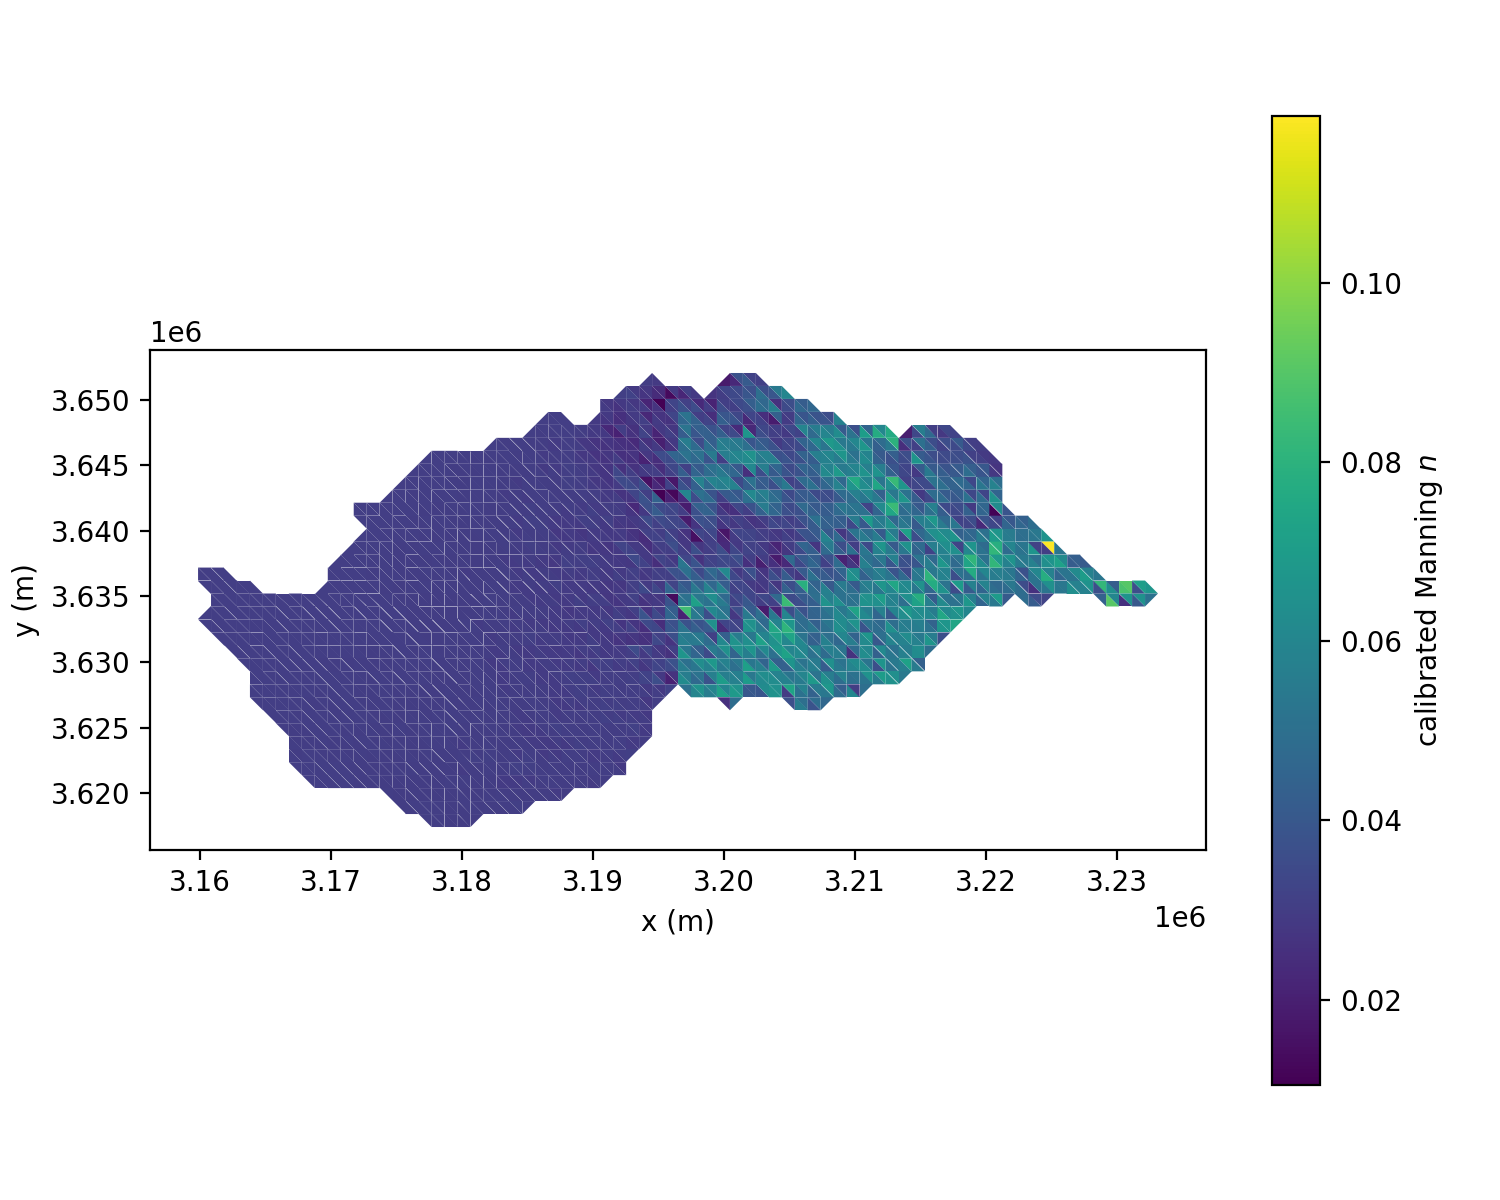
\includegraphics[width=0.24\linewidth]{houston_manning_300it.png}
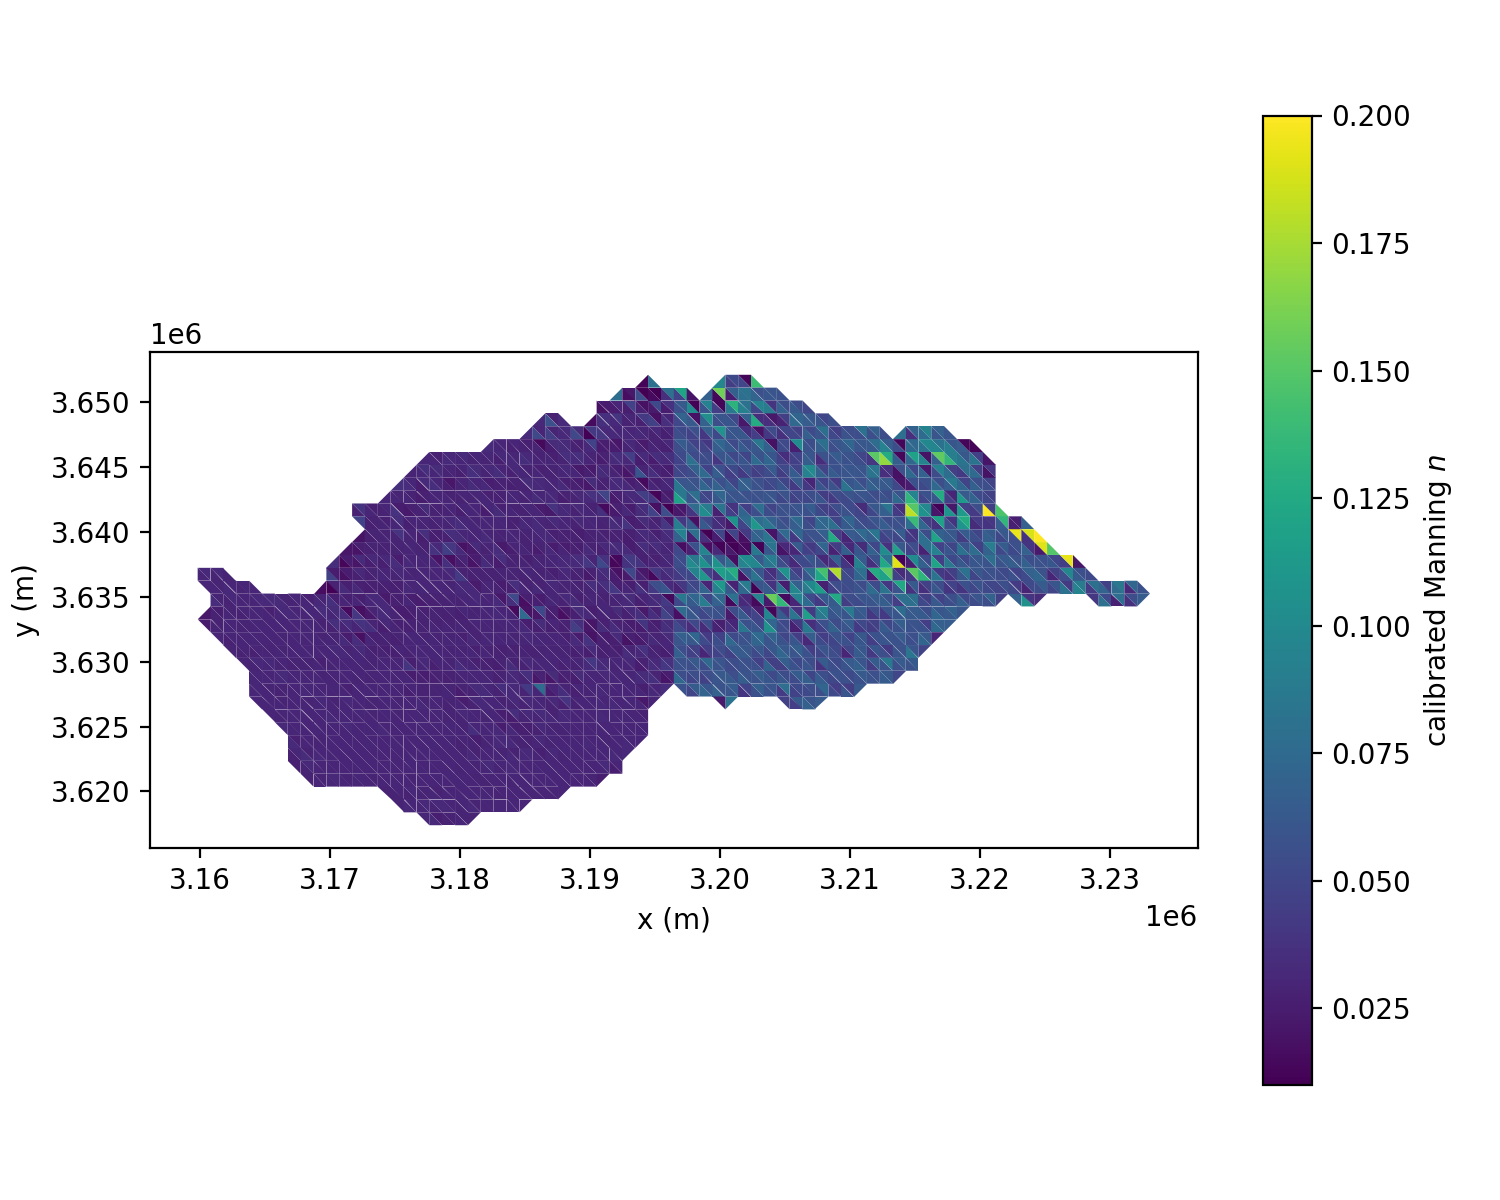
\includegraphics[width=0.24\linewidth]{houston_manning_2000it.png}
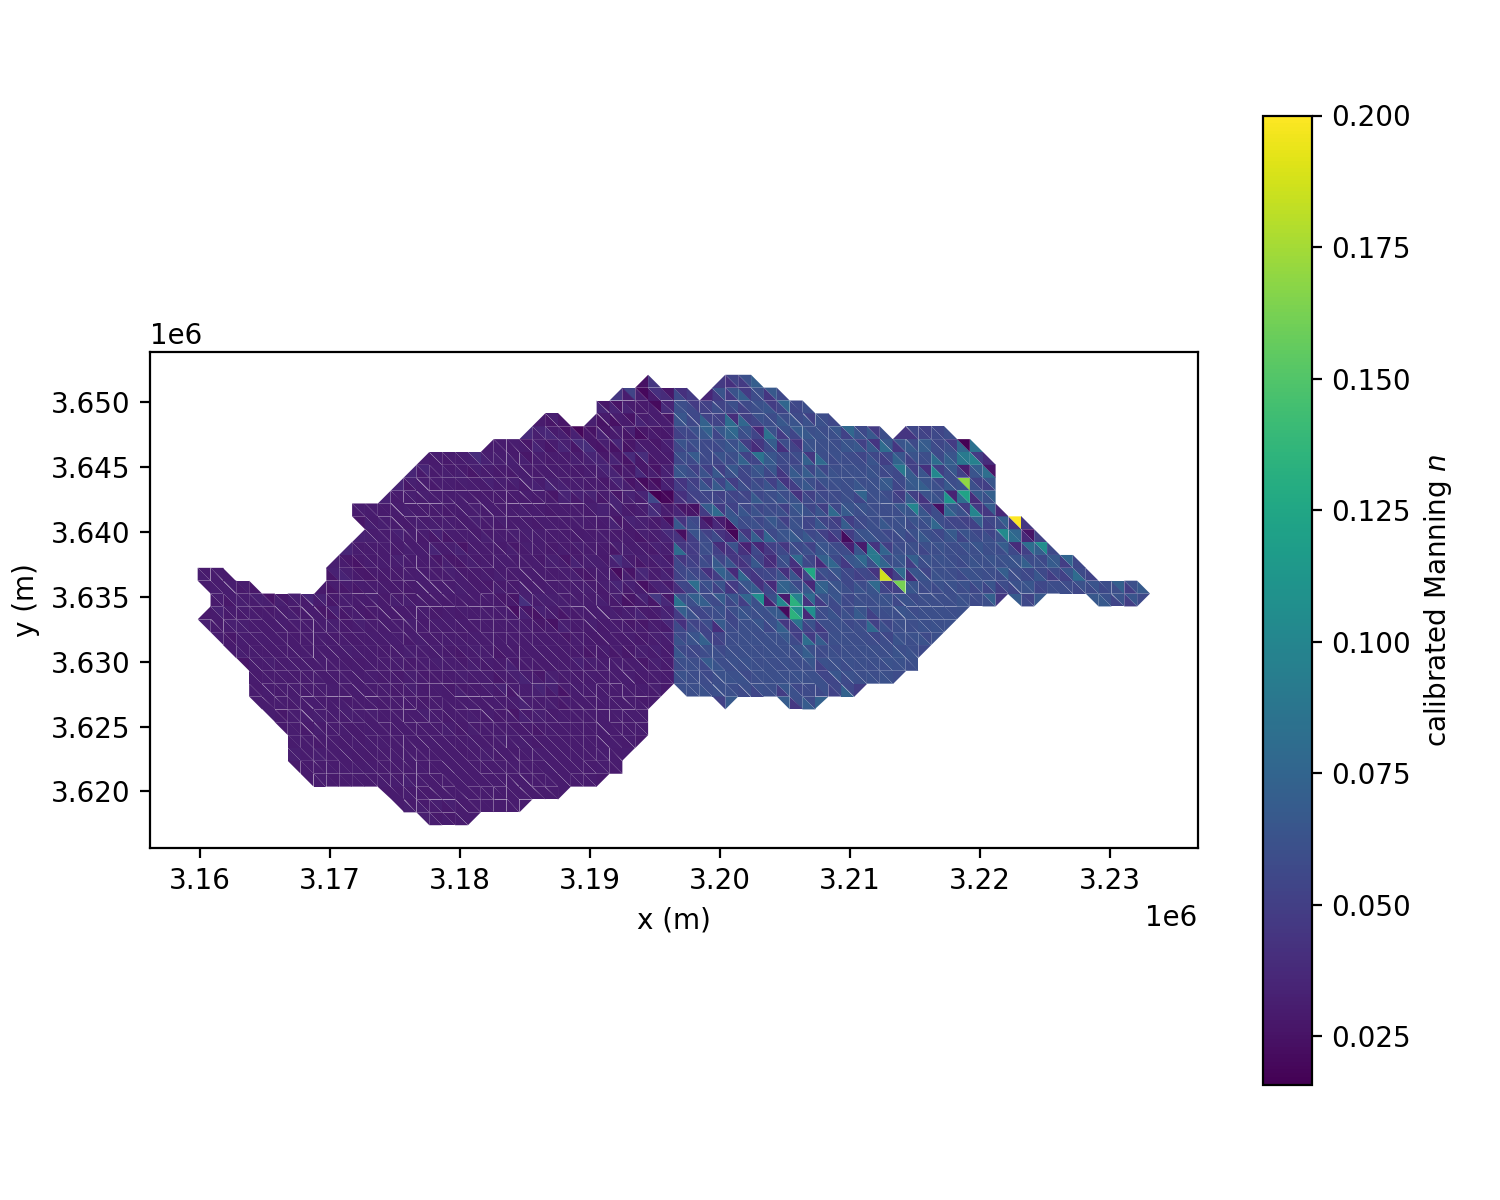
\includegraphics[width=0.24\linewidth]{houston_manning_reg.png}
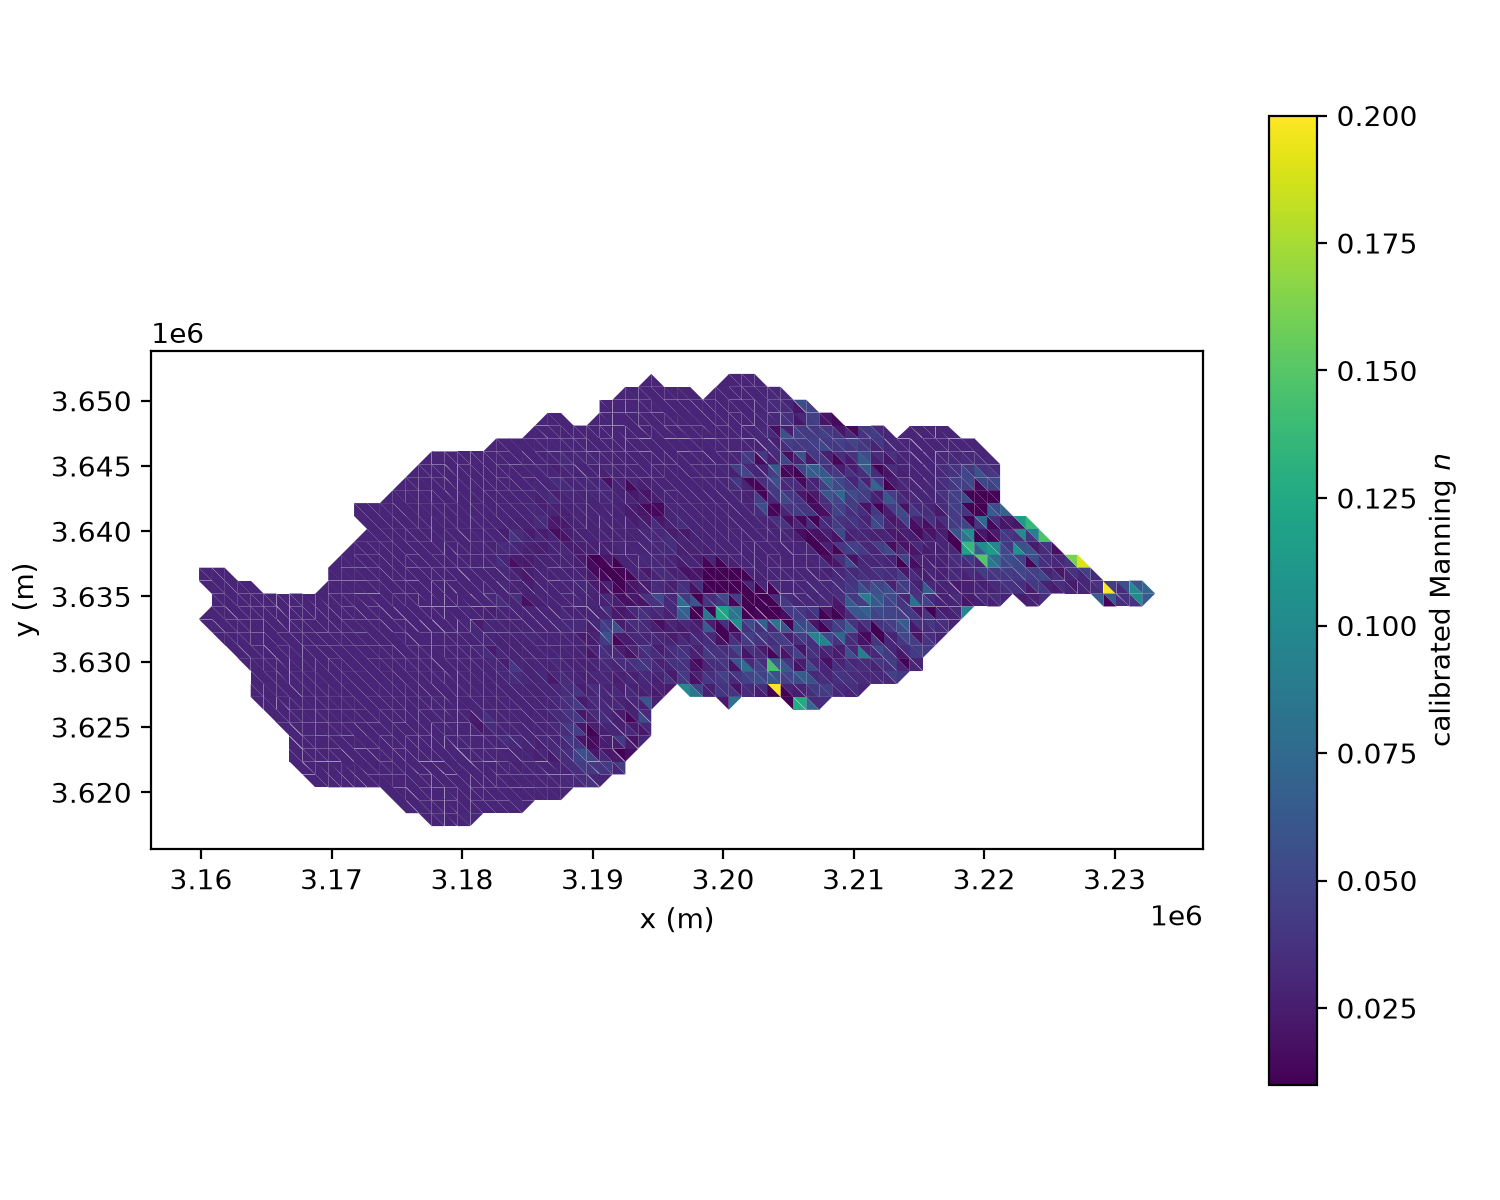
\includegraphics[width=0.24\linewidth]{houston_manning_real17.png}
\caption{Regularization, semiconvergence, and network density on the
Houston twin (2{,}746 parameters; truth: $n = 0.03$ west, $n = 0.06$
east of the midline; implicit stepping, 14 observation times). Far
left: weak regularization ($\beta = 10^{-5}$, 343 gauges) stopped
early at 300 iterations --- $26.3\%$ error. Center left: the same
setup run to 2000 iterations --- the misfit is lower but the field
drifts along unobserved directions to $38.0\%$ error and saturates the
bounds $[0.01, 0.2]$. Center right: proper Tikhonov weight
($\beta = 10^{-4}$, 686 gauges), 1000 iterations --- $19.4\%$ error,
no drift, sharp zone boundary. Far right: the \emph{real} network ---
the 17 in-mesh USGS gauges with Harvey stage records, same
$\beta = 10^{-4}$, 1000 iterations --- the misfit falls
$2\times10^{7}$-fold while the field recovers to only $44.9\%$: no
trace of the two-zone truth, near-prior almost everywhere with
null-space structure pinned against both bounds.}
\label{fig:map}
\end{figure}

\paragraph{The real gauge network.}
The synthetic gauge sets above are a controlled ramp; the network that
matters is the real one. Twenty USGS gauges fall inside the Houston
mesh, seventeen with Hurricane Harvey stage
records.\footnote{HydroShare DOI
\texttt{10.4211/hs.c037167e497546a1bc1508dfb32a9cff}.}
In the same twin with the observation operator built at those
seventeen gauge cells (238 observations, 17 gauges $\times$ 14 times,
against 2{,}746 parameters), BLMVM drives the misfit down by a factor
of $2\times10^{7}$ (the synthetic observations carry no noise and are
fit to roundoff) while the recovered field is $44.9\%$ from the truth
and saturates both bounds (Figure~\ref{fig:map}, far right). This is
semiconvergence in its purest form: the real network's null space is
so large that data fit says almost nothing about parameter recovery,
and no Tikhonov weight or stopping rule rescues a per-cell field from
238 observations. The practical conclusion for real-data calibration
is to shrink the parameter space to match the network. Shrinking it
is necessary and not sufficient, as the next subsection measures:
whether a reduced parameterization is identifiable depends on the
observation geometry and window, not on the ratio of observation to
parameter counts.

\subsection{Identifiability is a property of the observable: gauges
versus high-water marks at 30\,m}
\label{sec:identifiability}

The natural reduced parameterization for this domain is one Manning
value per NLCD land-cover class (15 classes at the 30\,m Turning mesh,
2.93M cells), with the published NLCD lookup as prior and truth for
twins. Counting favours it: even the sparse real network supplies an
order of magnitude more observations than parameters. Measurement
says otherwise. In a class twin on the 30\,m mesh at the real
13-gauge geometry (260 observations, a short early-transient window),
the objective falls $128\times$ while the recovered class values
remain $66\%$ wrong in relative $L^2$, worst class $81\%$. The
failure is structural: classes whose cells are dynamically distant
from every gauge (the three forest classes) never move from the
starting value, because within the window nothing their roughness
does reaches a gauge. The identical configuration observed at
418{,}076 strided cells recovers all fifteen classes to machine
precision, so the failure is the network, not the method. Fifteen
parameters and thirteen gauges, an ``overdetermined'' observation
count, remain unidentifiable.

The same question re-asked with the peak observable comes out
differently. Observing the same NLCD-truth twin at the 108
QC-passed high-water-mark cells (peak WSE sampled over a one-hour
rain-forced window, implicit stepping, free-outflow outlet;
Section~\ref{sec:hwm}) and calibrating fifteen classes from a uniform
start: the objective falls $81\times$, the peak-WSE error at the marks
drops from $0.103$\,m to $0.017$\,m MAE, and the area-dominant classes
are identified: the three developed-intensity classes, pasture, and
crops recover to $0.7$--$10.5\%$, together $83\%$ of the domain's
cells, for an area-weighted relative $L^2$ error of $0.20$ (unweighted
$0.58$). The residual errors concentrate in small-area classes
(forests, shrub, emergent wetland, $\sim$5\% of cells), which now
\emph{move} (they are sensitive, unlike in the gauge experiment) but
overshoot to the bounds along weakly constrained directions. That is
ordinary semiconvergence, treatable with regularization and longer
windows, rather than a structural absence of signal. Three caveats
apply: the one-hour window samples early-transient peaks, not flood
peaks (the real calibration windows are $6$--$12$ hours and should
only help); the run was capped at 15 quasi-Newton iterations; and
twin marks synthesized from the truth trajectory carry no
representation error, so this is an identifiability statement, an
upper bound on real-data performance rather than a forecast of it.

\paragraph{Noise turns identifiability into a signal-to-noise question.}
Every recovery above is noise-free, as are the verification twins
behind Section~\ref{sec:calibration}. Such experiments establish that
the gradient is right and that the observable carries the information;
they do not establish that a field can be calibrated from real data.
What separates the two is the size of the parameter-induced signal
relative to observation error, and that ratio moves by orders of
magnitude with the configuration (Table~\ref{tab:snr}). On a short
verification window the entire Manning-induced observation signal is a
few microns of water height, so a noise-free optimizer descends on it
indefinitely while a tenth of a millimetre of observation noise
destroys the recovery outright, and no Tikhonov weight in a sweep up
to $\beta = 1$ rescues it. At basin scale the same quantity is
$\sim$$0.1$\,m of peak water-surface elevation after one simulated
hour, five orders of magnitude larger, which is the regime in which a
parameter signal can exceed survey-grade high-water-mark error. The
lesson is not that the method is fragile: it is that friction must
act long enough to imprint a signal above the noise floor, which
makes window length a first-class calibration decision rather than a
cost parameter. The basin-scale noisy row shows what marginal
signal-to-noise looks like in practice, and why misfit at the marks
is the objective but not the result. With $0.15$\,m of observation
noise, even the \emph{true} field cannot beat a mark MAE of about
$\sigma\sqrt{2/\pi} \approx 0.12$\,m against the noisy values, and
the optimizer reaches that floor while driving five of the fifteen
classes onto their bounds (pasture, $428$k cells, to the ceiling) and
ending far from the true field it was supposed to recover. The data
fit is as good as truth could achieve; the parameters that achieve it
are wrong, because the last of the misfit was removed by matching
noise. On real data the parameter error is invisible and the
bound-pinning is its symptom, which is the argument for stronger
regularization, a longer window, and discrepancy-principle stopping
(stop at the noise level rather than descend past it) in the
production run.

\begin{table}
\centering\footnotesize
\begin{tabular}{@{}llp{2.6cm}p{5.9cm}@{}}
\toprule
Configuration & Signal & Observation noise & Outcome \\
\midrule
Verification twin & $5\,\mu$m & none & per-region recovery $4\times10^{-7}$ \\
(planar, 40 steps, & water & $0.1$\,mm & per-cell recovery destroyed ($0.20 \to 1.8$) \\
$1.8$\,s) & height & $1$\,mm & per-region destroyed ($4\times10^{-7} \to 0.83$, both at bounds) \\
\midrule
30\,m basin, 1\,h & $\sim$$0.1$\,m & none & area-weighted rel.\ $L^2$ $0.20$; MAE $0.103 \to 0.017$\,m \\
rain-forced, 108 marks & peak WSE & $0.15$\,m (HWM grade) & misfit falls $9.4\times$, MAE $0.23 \to 0.12$\,m --- but 5 of 15 classes pin to bounds \\
\bottomrule
\end{tabular}
\caption{Parameter-induced observation signal versus observation error.
The noise-free recoveries differ by seven orders of magnitude in the
signal they descend on; only the basin-scale row is a fair test against
survey-grade error ($0.1$--$0.3$\,m for high-water marks). Noise is a
deterministic, decomposition-independent perturbation of the twin
observations, so the comparison is reproducible across rank counts.}
\label{tab:snr}
\end{table}

\section{The real survey: what roughness can explain}
\label{sec:realsurvey}

The twins establish what the machinery can recover under controlled
conditions; this section turns it on the real Hurricane Harvey survey.
The observable changes first --- the stage gauges are unusable at this
resolution --- and everything after that is measured against surveyed
high-water marks: the uncalibrated baseline and the drainage defect it
exposes (Section~\ref{sec:hwm}), how much of the remaining error
roughness can remove (Section~\ref{sec:authority}), the calibration
(Section~\ref{sec:calibrated}), and the spectrum that counts how many
parameters the marks can actually determine
(Section~\ref{sec:spectrum}).
Section~\ref{sec:icauthority} then points the same measurement at the
initial condition.

\subsection{High-water marks and the uncalibrated baseline}
\label{sec:hwm}

Calibration against the actual stage records is blocked by geometry,
not software: at all 13 rain-driven USGS gauges in the 30\,m domain,
modelled water-surface elevation sits 1--11\,m \emph{above} observed
stage, because a 30\,m cell stores one mean ground elevation ---
the bank of an incised bayou --- while the gauge hangs in
the channel below it; the offset is time-varying as the real channel
fills, so no per-gauge datum correction can repair it. Comparing the
mesh directly against the stage record makes the geometry explicit
(Table~\ref{tab:gauges}): over the calibration window the cell bed
sits above the \emph{peak} observed water surface at seven of the
twelve gauges with data, and above the water surface for $71\%$ of all
gauge-hours. Only the two Buffalo Bayou main-stem gauges, where the
channel is wider than a cell, and the two gauges in the Addicks and
Barker reservoir pools hold their water for the whole window. The
mesh resolves the major channel and not the tributaries, which is
where nine of the thirteen gauges sit.
\paragraph{Calibrating on the gauges instead.}
The four gauges that hold their water for the whole window are enough
to pose the calibration the other way round, and doing so tests
whether a roughness field fitted to one observable predicts the other.
We calibrated the same three classes on the above-bed gauge stage
(134 observations, an observation counting only while the observed
water surface is above the cell bed) and scored the result on the 46
marks. The answer is that it does not, and the failure is
directional rather than marginal (Table~\ref{tab:crossobs}). The
gauge calibration raises all three classes --- developed-low and
developed-medium to the $3\times$ upper bound, woody wetland to
$1.74\times$ --- where the mark calibration puts the latter two on the
$0.3\times$ floor. The two observables place the same class a factor
of ten apart, each at an edge of the same prior. Scored on the marks,
the gauge-calibrated field reaches $0.7609$\,m against the
uncalibrated prior's $0.7188$: \emph{calibrating on the gauges makes
the model worse at the marks than not calibrating at all}, while
lowering the gauge misfit by $23\%$.

The mechanism is the geometry of the preceding paragraph. At a mark on
the floodplain the modelled peak is too high, so the misfit gradient
asks for less conveyance; at a gauge on a bank cell the modelled stage
is too low by the representation offset, so it asks for more. Neither
request is about friction. The gauge residual is the size of that
offset rather than of a roughness error: at the NLCD prior the
above-bed gauge misfit is $3.24$\,m RMSE, and the best field we
obtained against it leaves $2.84$\,m, so roughness spans $12\%$ of a
discrepancy that a $30$\,m mesh of an incised channel would produce
with no friction error at all. A calibration reported against the
gauges alone would show a $23\%$ misfit reduction and a physically
impossible field.

We report this as the paper's validation result. It is negative, and
it is the one the survey-only numbers of
Section~\ref{sec:calibrated} need: a three-parameter field that
removes $12.5\%$ of the mark error does not transfer to a second
observable in the same basin and window, so that $12.5\%$ is a fit and
not a skill. The two observables agree on one thing, that the
land-cover table is not where this model's error lives.

\begin{table}
\centering\small
\begin{tabular}{@{}lrrrrr@{}}
\toprule
Manning field & 22 & 23 & 90 & gauge $J$ & mark MAE \\
\midrule
NLCD lookup & $0.090$ & $0.120$ & $0.098$ & $31{,}313$ & $0.7188$ \\
calibrated on the gauges & $0.27$ & $0.36$ & $0.171$ & $24{,}007$ & $0.7609$ \\
calibrated on the marks & $0.210$ & $0.036$ & $0.029$ & $30{,}333$ & $0.6290$ \\
\bottomrule
\end{tabular}
\caption{The same three classes (developed-low 22, developed-medium 23,
woody wetland 90) calibrated against each observable and scored against
both, at $\sigma_\alpha = 0.30$ with the other twelve classes frozen at
the lookup. Manning $n$ in $\mathrm{s\,m^{-1/3}}$, gauge $J$
over 134 above-bed stage observations, mark MAE in metres over the 46
cluster-A marks. Each calibration improves its own observable and the
gauge calibration degrades the other, past the uncalibrated prior. The
bound is $\alpha \in [0.3, 3]$, so $0.27$ and $0.36$ are at it.}
\label{tab:crossobs}
\end{table}

\begin{table}
\centering\small
\begin{tabular}{@{}lrrr@{}}
\toprule
Gauge & cell bed (m) & window WSE (m) & above bed \\
\midrule
Buffalo Bayou nr Katy & $33.27$ & $35.56$--$36.05$ & $100\%$ \\
Buffalo Bayou at Houston & $6.93$ & $10.64$--$12.77$ & $100\%$ \\
Langham Ck nr Addicks & $28.23$ & $30.70$--$31.28$ & $100\%$ \\
Bear Ck nr Barker & $34.73$ & $34.96$ & $100\%$ \\
Buffalo Bayou nr Fulshear & $31.47$ & $31.23$--$31.56$ & $29\%$ \\
Langham Ck at W Little York & $34.10$ & $32.76$--$34.09$ & $0\%$ \\
S Mayde Ck & $34.60$ & $34.07$--$34.29$ & $0\%$ \\
Whiteoak Bayou at Alabonson & $23.60$ & $22.26$--$23.48$ & $0\%$ \\
Brickhouse Gully & $20.40$ & $16.24$--$19.64$ & $0\%$ \\
Cole Ck & $25.30$ & $20.95$--$22.51$ & $0\%$ \\
Little Whiteoak Bayou & $14.50$ & $10.65$--$13.37$ & $0\%$ \\
Whiteoak Bayou at Main St & $11.80$ & $9.66$--$11.33$ & $0\%$ \\
Whiteoak Bayou at Houston & $15.03$ & \multicolumn{2}{l}{no record in window} \\
\bottomrule
\end{tabular}
\caption{The 30\,m mesh against the stage record at the thirteen
rain-driven USGS gauges over the calibration window (event hours
29--41). Stage at these gauges is published as water-surface elevation
(WSE) in NAVD88, the datum of the mesh, so the cell's mean bed
elevation and the observed water surface compare directly. ``Above
bed'' is the fraction of the window's 15-minute records with the
observed water surface above the cell bed. At seven gauges the bed
sits above even the window's peak stage: the cell holds the bank, and
no roughness value places water in it at the elevation the gauge
reads.}
\label{tab:gauges}
\end{table}
We therefore
changed the observable to the USGS high-water-mark archive: surveyed
\emph{peak} water-surface elevations on structures and debris lines,
i.e.\ on the floodplain surfaces a 30\,m cell does represent, and the
benchmark currency of the flood-modeling literature (Inunda reports
$0.67$\,m MAE against Harvey high-water marks~\cite{li2026inunda}).
Of 2{,}364 Harvey marks, 324 fall in the Turning domain; applying to
the marks the same QC that disqualified the gauges --- is the surveyed
elevation above the containing cell's bed? --- rejects $62\%$ of them
(they are channel surveys), leaving 108 marks of quality fair or
better. The mismatch this QC addresses is the one Xu et al.\ measured on
a 30\,m simulation of the same event: validated against 48 marks, their
simulation had an RMSE of $0.9$\,m with 25 of 48 within $25\%$, which they
attribute to comparing a point survey with a cell average~\cite{xu2025harvey}.
Two choices here reduce that exposure. The QC keeps only marks on surfaces
a cell represents, and the misfit compares water-surface elevations rather
than depths, so the difference between the ground at the point and the
mean ground of the cell enters once, through the cell bed, and not a
second time through the depth. The misfit compares each mark cell's peak simulated WSE over
the window, $\max_k H u(t_k)$, against the surveyed value; its
adjoint needs no new machinery, because each mark's residual can be
injected at its own argmax time in the segmented backward sweep of
Algorithm~\ref{alg:sweep}, which is the exact gradient wherever the
peak time is locally constant. The
parameter gradient of the peak misfit passes the same central-difference
gates as every other block on the smooth verification twin. At basin
scale the naive check fails, and a set of instrumented measurements
pins down why, in a way that validates the gradient rather than the
check (Table~\ref{tab:fdwindow}). No mark's argmax moves and none
flips wet/dry across any probe, so the discrepancy lives below the
observable; the evaluations are deterministic to nine digits and the
FD value is stable across a decade of probe step, which excludes
noise, curvature truncation, and sparse kinks. Decisively, the gap
\emph{accumulates with trajectory length}: at the shortest window the
gate passes at the inner-solve floor with every piece of machinery
engaged, and it grows three orders of magnitude by basin window
lengths. A proportional defect in $\partial f/\partial n$ or the
adjoint accumulation would err the same fraction at any window length;
trajectory-accumulated branch crossings --- the probe shifts which
cells cross the depth cutoff at some step --- predict exactly this
profile. Two further checks close it: as the probe shrinks, the FD
converges to the adjoint direction by direction --- the largest
single-class direction passes the $10^{-5}$ gate outright at the
smallest probe --- and the fifteen per-class gaps \emph{sum} to the
domain-wide gap, the additivity that independent per-cell branch
crossings predict and no plausible defect would arrange. The measured
conclusion: the adjoint returns the exact one-branch derivative; over
long windows the objective is dense with wet/dry branch surfaces, and
a finite-step central difference converges to a locally
\emph{smoothed} slope that sits several percent from any one branch. The quasi-Newton iteration consumes one-branch
derivatives of a piecewise-smooth objective --- standard practice for
$\max$-type and switching systems --- and its observed descent
(Section~\ref{sec:identifiability}) is consistent with that footing.

\begin{table}
\centering\small
\begin{tabular}{@{}lrl@{}}
\toprule
Window & Steps & FD-vs-adjoint gap, domain-wide direction \\
\midrule
smooth verification twin & 40 & $9\times10^{-7}$ (gate $10^{-5}$: pass) \\
basin, 1 min & 60 & $9\times10^{-5}$ (inner-solve floor: pass) \\
basin, 5 min & 300 & $8\times10^{-3}$ \\
basin, 15 min & 900 & $2\times10^{-2}$ \\
basin, 30 min & 1800 & $2\times10^{-1}$ \\
basin, 1 h & 3600 & $7\times10^{-2}$ \\
\bottomrule
\end{tabular}
\caption{The FD gate's failure accumulates with trajectory length on
identical basin, rain, marks, and converged tolerances --- the
signature of branch crossings along the trajectory, not of gradient
error. The 30-minute and 1-hour rows sample peaks over different
horizons, so strict monotonicity across them is not expected;
single-class directions sit one to three orders lower at every
window.}
\label{tab:fdwindow}
\end{table}
The remaining scientific choice is the calibration window, which for
marks that record the event maximum must cover the flood peak.

\paragraph{The uncalibrated baseline against the real survey.}
Because the marks record the event maximum, the baseline evaluation
must simulate through the crest: a 72-hour rain-forced
forward from the available initial state (2017-08-26 18:00, reaching
past the Buffalo Bayou crest), NLCD-prior Manning, free outflow,
backward Euler at $\Delta t = 1$\,s on the 2.93M-cell mesh ---
259{,}200 implicit steps, \emph{zero} Newton failures, two hours on
one GPU node. The model wets all 108 marks, and the uncalibrated
peak-WSE error decomposes into two distinct populations
(Table~\ref{tab:baseline}; confirmed mark for mark at fully converged
inner tolerances). The marks that crest inside the window carry the
error a Manning field can plausibly address. The others never crest at
all: their cells fill monotonically through the entire window ---
every one peaks at the final hour with zero recession, still rising
while the first population is already draining --- accumulating some
ten metres of standing water whose late-window inflow arrives
laterally, after the rain has ended. Those cells sit in the downstream
Buffalo Bayou reach: the model cannot drain it, a conveyance/outlet
defect that no roughness value can absorb and that would corrupt any
calibration asked to fit it. The obvious suspicion --- that we simply
failed to give the domain an exit --- does not survive inspection of
the mesh. The domain is a delineated watershed rather than a
rectangular cutout ($35$ of its $6{,}198$ boundary nodes lie on the
bounding box), so its unflagged perimeter is a catchment divide and a
reflecting wall is the right condition there; and its single
free-outflow side set sits at the perimeter's lowest point, the only
boundary nodes at $z \approx 0$ against a boundary median of
$29.9$\,m. The exit is present and correctly placed. What the ponded
reach then reveals is a limitation of the idealization itself: it
holds water above the elevation of parts of its own divide, which a
reflecting wall retains and the real event would have spilled.

Three measurements on the 72-hour forward make that concrete. The 37
never-cresting mark cells are not local depressions in the terrain:
one of the 37 is lower than every edge-neighbour, against six of the
71 marks that crest normally. Rainfall is not what fills them: on the
basin-mean MRMS series, simulation hours 60--72 carry $1.7\%$ of the
event's rain and the hours beyond 72 carry none. What the model holds
there is a lake. Its peak water surface across all 37 cells is
$20.0 \pm 1.1$\,m, over surveyed peaks that run from $6.2$ to $20.2$\,m
and beds from $0.3$ to $18.2$\,m: the surveyed water surface slopes
toward the outlet and the modelled one does not (the correlation of
surveyed WSE with the model's excess is $-0.93$, and a flat pond at
$20.3$\,m predicts that excess to $1.1$\,m RMS). The divide sets the
level. A quarter of the perimeter's $6{,}198$ nodes, all in the
domain's eastern quarter, lie below $20$\,m, while the free-outflow
side set is thirteen element edges wide: the real flood left across
the low divide, and the model can leave only through the outlet, so
it ponds to the height its walls impose. The calibration target is therefore the
71 admissible marks; the drainage defect is reported as a finding in
its own right; and the remaining bundle (initial-condition, rainfall,
mesh-elevation, and datum error) is what the calibration must be
prevented from absorbing along with the roughness signal. The
literature's calibrated benchmark on this event is $0.67$\,m
MAE~\cite{li2026inunda}.

\begin{table}
\centering\small
\begin{tabular}{@{}lrrr@{}}
\toprule
Marks & $n$ & MAE & bias \\
\midrule
crest inside the 72-h window & 71 & $1.51$\,m & $+1.20$\,m \\
never crest (reach cannot drain) & 37 & $7.06$\,m & $+7.06$\,m \\
all & 108 & $3.41$\,m & $+3.21$\,m \\
\bottomrule
\end{tabular}
\caption{The uncalibrated baseline against the 108 surveyed high-water
marks, decomposed. The second population is model-high at every single
mark and identifies a reach with no working exit; the first is the
calibration target.}
\label{tab:baseline}
\end{table}

\paragraph{The defect is a gradient, not a switch.}
Sorting the marks by crest time splits them into three groups, and
those groups turn out to be three \emph{spatial bands} whose bias
increases monotonically downstream (Table~\ref{tab:bands}). The
never-crest population is the end of a continuum, not a separate
pathology: the intermediate band already carries $+2.85$\,m of the
same model-high signature. Two consequences follow. First, a
calibration window has to be placed on the upstream band, where the
model is physically sound --- crests there fall in event hours
29--41, and the 46 marks in that band are the target of every
production number below. Second, the intermediate band is
\emph{not} clean held-out data, which rules out the obvious
validation design; out-of-sample skill has to be tested by
cross-validation within the upstream band instead.

\begin{table}
\centering\small
\begin{tabular}{@{}lrrrr@{}}
\toprule
Group & $n$ & mean lon. & bias & MAE \\
\midrule
crest h29--41 (upstream) & 46 & $-95.695$ & $+0.30$\,m & $0.72$\,m \\
crest h48--72 (middle) & 25 & $-95.568$ & $+2.85$\,m & $2.96$\,m \\
never crest (downstream) & 37 & $-95.440$ & $+7.06$\,m & $7.06$\,m \\
\bottomrule
\end{tabular}
\caption{The crest-timing groups are spatial bands, and the model-high
bias grows monotonically downstream toward the reach with no working
exit. The upstream band is the calibration target; the middle band is
contaminated by the same defect at intermediate strength and cannot
serve as held-out data.}
\label{tab:bands}
\end{table}

\subsection{How much of the error can roughness explain?}
\label{sec:authority}

Before asking an optimizer to fit fifteen land-cover classes it is
worth asking what any roughness field could achieve, and that question
has an optimizer-independent answer. Scaling the entire NLCD field by
a single factor $\alpha$ traverses the natural first direction of the
problem --- close to, though as Section~\ref{sec:spectrum} measures,
not exactly, its most identifiable one; evaluating the peak-WSE misfit
along it bounds what this paper calls the \emph{authority} of a
parameter over an observable: the amount of the model--survey error
that changing the parameter can remove, measured without reference to
how, or whether, a calibration converges. The largest such amount over
the parameter's defensible range is the parameter's \emph{ceiling}.
Both are lengths, in metres, and fractions of the uncalibrated error,
and the paper uses the two words in that sense only.

We ran that scan on the production configuration: a 12-hour window over
the upstream crest cluster (event hours 29--41), initialized from an
hourly checkpoint of the 72-hour forward and with the rain re-aligned
to the window start (both validated bit-exactly), scored against the 46
surveyed marks whose modelled crest falls inside the window. Each point
is one forward with no adjoint (Table~\ref{tab:alpha}).

\paragraph{The window is set by the observable.}
A high-water mark records an event maximum, so it carries information
about roughness only if its crest occurs inside the calibration window;
before its crest it is an inequality, and after it a constant. The
measured crest times decide the window rather than any budget: they are
bimodal, clustering in event hours 29--42 and 60--72 with an empty gap
between, so a window spanning both would spend most of its length
integrating marks that had already peaked. The upstream cluster is also
the population the model can legitimately be scored against at all,
since the downstream marks sit in a reach it cannot drain
(Section~\ref{sec:hwm}) --- a defect no window length repairs. The 46
marks used throughout this paper are therefore those for which the
observable means what it is meant to mean, and every number reported
here --- the uncalibrated baseline, the scans, and the calibration ---
is measured on that same window, so they compose --- including the
spectrum of Section~\ref{sec:spectrum}.

\begin{table}
\centering\small
\begin{tabular}{@{}lllrr@{}}
\toprule
$\alpha$ & $n$ range & $J$ & MAE & dry \\
\midrule
$0.20$ & $0.005$--$0.032$ & \multicolumn{3}{l}{implicit solve diverges} \\
$0.30$ & $0.008$--$0.048$ & $6.737\times10^{2}$ & $0.6392$ & 1/46 \\
$0.45$ & $0.012$--$0.072$ & $7.038\times10^{2}$ & $0.6614$ & 1/46 \\
$0.60$ & $0.016$--$0.096$ & $7.406\times10^{2}$ & $0.6776$ & 1/46 \\
$0.70$ & $0.019$--$0.112$ & $7.655\times10^{2}$ & $0.6894$ & 1/46 \\
$0.80$ & $0.022$--$0.128$ & $7.813\times10^{2}$ & $0.6991$ & 0/46 \\
$1.00$ (NLCD) & $0.027$--$0.160$ & $8.083\times10^{2}$ & $0.7188$ & 0/46 \\
\bottomrule
\end{tabular}
\caption{Uniform roughness scan on the production configuration
(12-hour window, 46 cluster-A marks); every cell carries
$n = \alpha\,n_{\rm NLCD}$, so the \emph{n} range column is the whole
lookup table scaled by $\alpha$. $J$ falls monotonically toward
lower roughness with no interior minimum: the entire uniform-roughness
knob is worth $0.08$\,m against a $0.72$\,m error, and only at roughness
$30\%$ of published values, where $n$ reaches $0.008$ and smooth
concrete is $\approx 0.012$. Within a defensible range it is worth about
$3$\,cm ($\alpha = 0.70$, itself the optimum implied by the prior width
of Section~\ref{sec:calibration}). The limit at $\alpha = 0.2$ is
numerical, not drying --- one mark stays dry throughout.}
\label{tab:alpha}
\end{table}

\begin{figure}[t]
\centering
% The authority figure: what each parameter can do to the peak-WSE error.
%
% Form: a line chart -- the data's job is change over a continuous parameter,
% and both series share BOTH axes honestly. x is a multiplicative factor on the
% parameter (alpha = n/n_prior for roughness, a = scale on the initial state),
% y is the same peak-WSE MAE in metres over the same 46 marks. That shared
% meaning is what makes one axis correct here; a dual-axis version would be
% meaningless.
%
% Both curves pass through the same point at 1.0 (the uncalibrated model), so
% the reader's eye lands on a shared anchor and the slopes do the arguing.
%
% Colour: categorical slots 1 and 2 of the validated palette (blue #2a78d6,
% orange #eb6834; adjacent-pair CVD dE 24.7 protan, 33.6 normal -- all six
% checks pass). Identity is never carried by colour alone: each series also has
% a distinct marker and dash pattern, so the figure survives greyscale printing.
%
% NB the axis spans 0.25-1.25 because the ROUGHNESS scan runs down to 0.30 --
% an earlier draft set xmin at 0.55 with clip=false and silently drew that
% curve outside the axis box.
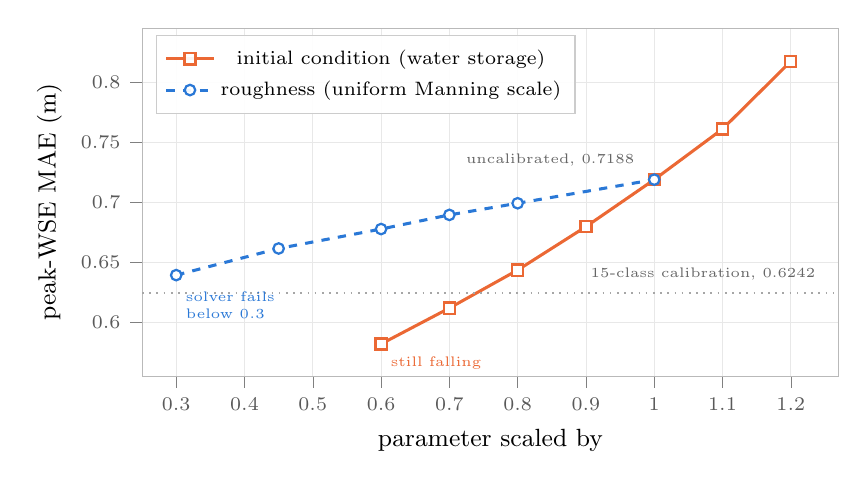
\begin{tikzpicture}
\begin{axis}[
  width=0.86\linewidth, height=6.0cm,
  xlabel={parameter scaled by},
  ylabel={peak-WSE MAE (m)},
  xmin=0.25, xmax=1.27,
  ymin=0.555, ymax=0.845,
  xtick={0.3,0.4,0.5,0.6,0.7,0.8,0.9,1.0,1.1,1.2},
  xticklabel style={/pgf/number format/fixed, /pgf/number format/precision=1},
  ytick={0.60,0.65,0.70,0.75,0.80},
  yticklabel style={/pgf/number format/fixed, /pgf/number format/precision=2},
  tick align=outside, tick pos=left,
  axis line style={gray!55},
  tick label style={font=\scriptsize, color=black!65},
  label style={font=\small},
  grid=major, grid style={gray!18, line width=0.3pt},
  legend style={font=\scriptsize, at={(0.02,0.98)}, anchor=north west,
                draw=gray!40, fill=white, fill opacity=0.93, text opacity=1,
                row sep=0.5pt, inner sep=3pt},
]

% --- initial condition: a scale on antecedent water storage (velocities fixed)
\addplot[color={rgb,255:red,235;green,104;blue,52}, line width=1.1pt,
         mark=square*, mark size=2.0pt, mark options={fill=white, line width=0.8pt}]
  coordinates {(0.6,0.5818) (0.7,0.6117) (0.8,0.6434) (0.9,0.6796)
               (1.0,0.7188) (1.1,0.7610) (1.2,0.8174)};
\addlegendentry{initial condition (water storage)}

% --- roughness: a uniform scale on the NLCD Manning field
\addplot[color={rgb,255:red,42;green,120;blue,214}, line width=1.1pt,
         dashed, mark=*, mark size=1.9pt,
         mark options={solid, fill=white, line width=0.8pt}]
  coordinates {(0.30,0.6392) (0.45,0.6614) (0.60,0.6776) (0.70,0.6894)
               (0.80,0.6991) (1.00,0.7188)};
\addlegendentry{roughness (uniform Manning scale)}

% --- the calibrated field: off both curves, since it redistributes
\addplot[gray!70, line width=0.6pt, dotted, forget plot]
  coordinates {(0.25,0.6242) (1.27,0.6242)};
\node[font=\tiny, color=black!60, anchor=south east]
  at (axis cs:1.25,0.6265) {15-class calibration, 0.6242};

% --- the shared anchor
\node[font=\tiny, color=black!60, anchor=south east]
  at (axis cs:0.985,0.7215) {uncalibrated, 0.7188};

% --- why each curve stops where it does
\node[font=\tiny, color={rgb,255:red,42;green,120;blue,214},
      anchor=north west, align=left]
  at (axis cs:0.30,0.6330) {solver fails\\below $0.3$};
\node[font=\tiny, color={rgb,255:red,235;green,104;blue,52},
      anchor=north west, align=left]
  at (axis cs:0.60,0.5790) {still falling};
\end{axis}
\end{tikzpicture}

\caption{What each parameter can do to the peak-WSE error, on identical
axes: the horizontal axis scales the parameter, the vertical axis is the
same mean absolute error over the same 46 marks, and both curves pass
through the uncalibrated model at $1.0$. Roughness is concave and runs
out --- and its useful end is physically indefensible, reaching
$n = 0.008$ before the implicit solve fails. The initial condition is
about four times steeper per unit fractional change, convex, and has not
turned over at a $40\%$ reduction in antecedent water. The dotted line is
the fifteen-class calibration, which lies off both curves because it
redistributes roughness rather than scaling it.}
\label{fig:authority}
\end{figure}

\textbf{The entire uniform-roughness knob is worth $0.08$\,m against a
$0.72$\,m error} (Figure~\ref{fig:authority}) --- about $11\%$ --- and it reaches that only at
$\alpha = 0.3$, i.e.\ Manning values $30\%$ of the published NLCD
lookup, as low as $n = 0.008$ where smooth concrete is $\approx 0.012$.
Over a physically defensible range ($\alpha \gtrsim 0.7$) the knob is
worth about three centimetres. The curve is mildly concave with no
interior minimum: $J$ falls monotonically toward lower roughness until
the implicit solve fails.

That number is corroborated from an independent direction. The
identifiability twin of Section~\ref{sec:identifiability} measured the
peak-WSE signal induced by a large class perturbation at
$\sim 0.1$\,m --- the same authority scale, from a different
experiment. So $85$--$90\%$ of the model-versus-survey residual is not
roughness at all: it is rainfall forcing, mesh elevation, datum, and
representation error at 30\,m.

\paragraph{The observable constrains one mode, not fifteen.}
A natural objection is that spatial redistribution should beat uniform
scaling --- that fifteen classes have freedom a single $\alpha$ does
not. We tested it directly by scaling only part of the domain to
$\alpha = 0.45$ and leaving the rest at the NLCD prior
(Table~\ref{tab:halves}).

\begin{table}
\centering\small
\begin{tabular}{@{}lrrrr@{}}
\toprule
Field & $J$ & $\Delta J$ & MAE & $\Delta$MAE \\
\midrule
NLCD prior & $808.3$ & --- & $0.7188$ & --- \\
developed classes 21--24 only ($71.6\%$ of cells) & $786.8$ & $-21.5$ & $0.7306$ & $+0.0118$ \\
everything else ($28.4\%$) & $827.5$ & $+19.2$ & $0.7268$ & $+0.0080$ \\
both (= uniform $\alpha = 0.45$) & $703.8$ & $-104.5$ & $0.6614$ & $-0.0574$ \\
\bottomrule
\end{tabular}
\caption{Each half of the domain scaled alone makes the fit
\emph{worse}; scaled together they help by $45\times$ the sum of the
parts. Peaks are set by path-integrated conveyance along flow paths
that cross both groups, so only domain-coherent changes drain them.}
\label{tab:halves}
\end{table}

Each half alone makes the fit \emph{worse}, and the two together help
by $45\times$ the sum of the parts --- a strong positive interaction,
not two competing signs. The mechanism is consistent with every other
measurement: a mark's peak is set by the \emph{path-integrated}
conveyance from upstream to that mark, and those paths cross both
groups. Speeding part of a path does not drain it; the resulting
fast/slow junction ponds water, so partial changes \emph{raise} peaks.
Only a domain-coherent change lowers them.

The conclusion is a design finding, not a tuning observation. The
peak-WSE observable at these marks constrains \emph{one} roughness
degree of freedom at the prior width used here --- the domain-scale,
path-integrated conveyance --- worth $\sim 10\%$ of the model--survey
discrepancy, and about three at a $\pm 30\%$ width
(Section~\ref{sec:spectrum}). It
does not carry fifteen classes' worth of information. This unifies the
earlier evidence rather than sitting beside it: the perfect-data twin
recovers only the classes that move the domain mean, and the noisy twin
pins the others to bounds precisely because they carry no signal to
fit, so the optimizer fits noise in those directions instead.

\paragraph{Relation to equifinality.}
None of this is a new phenomenon: that many different parameter sets
reproduce a hydrological observation about equally well is Beven's
equifinality thesis~\cite{beven1992glue,beven2006equifinality}, and the
usual response is to characterize the acceptable set by sampling it.
What an adjoint changes is the cost of the diagnosis. Where GLUE-style
methods \emph{sample} the equifinal set with many forward runs, the
measurements above \emph{measure} its dominant direction directly:
four forward evaluations bound the authority of the whole roughness
field, and two more show that the modes are not separable. The result
is the same kind of statement, obtained at a cost that does not grow
with the number of parameters --- which is what makes it affordable
before a calibration rather than after one.

\paragraph{Why this generalizes.}
The measurement uses nothing specific to roughness. Given a
parameter, an observable, and a model error to explain, the same three
steps --- scan the dominant parameter direction, check whether
sub-domain changes are separable, and compare the resulting authority
against the residual --- bound what calibrating that parameter can
ever accomplish, before any optimizer is written. We suggest it as a
routine precondition for calibration studies, which commonly report the
misfit reduction achieved without establishing the ceiling it was
approaching.

\subsection{The calibration against the real survey}
\label{sec:calibrated}

The scan sets the bar a multi-parameter calibration must clear to
justify its parameters. Running the class calibration of
Section~\ref{sec:calibration} on the same configuration --- fifteen NLCD
classes, relative variables, prior width as discussed below, starting
from the NLCD lookup --- clears it (Table~\ref{tab:ladder}).

\begin{table}
\centering\small
\begin{tabular}{@{}lrrl@{}}
\toprule
Manning field & MAE & $\Delta$ & physically defensible? \\
\midrule
NLCD lookup (uncalibrated) & $0.7188$ & --- & yes, by construction \\
uniform $\alpha = 0.70$ & $0.6894$ & $-0.029$ & yes \\
uniform $\alpha = 0.30$ & $0.6392$ & $-0.080$ & no ($n$ to $0.008$) \\
calibrated, 15 classes, $\sigma_n = 0.015$ & $0.6116$ & $-0.107$ & mostly; one class at a bound \\
calibrated, 15 classes, $\sigma_\alpha = 0.30$ & $0.6154$ & $-0.103$ & no; two classes at the floor \\
calibrated, 3 classes, $\sigma_n = 0.015$ & $0.6274$ & $-0.091$ & no; two classes at the floor \\
calibrated, 3 classes, $\sigma_\alpha = 0.30$ & $0.6290$ & $-0.090$ & no; two at the floor, one at $2.3\times$ \\
calibrated, 3 classes, $\sigma_\alpha = 0.50$ & $0.6295$ & $-0.089$ & no; all three at a bound \\
\bottomrule
\end{tabular}
\caption{Peak-WSE MAE against the 46 cluster-A marks. Both fifteen-class
calibrations beat the entire uniform-roughness knob --- including its
physically indefensible end --- and beat the best \emph{defensible}
uniform field by $0.078$\,m; spatial redistribution is worth about three
and a half times what a single global scale can reach. The
$\sigma_n = 0.015$ field took nine quasi-Newton iterations, the
$\sigma_\alpha = 0.30$ field three, and they agree in misfit to four
figures ($J_{\rm mis} = 615.4$), which suggests a floor that roughness
does not set. The three-class rows are the calibration
Section~\ref{sec:spectrum} selects: their MAE moves by $0.002$\,m across
a threefold change in prior width, and their two best-informed classes
land on the floor under all three.}
\label{tab:ladder}
\end{table}

Two things qualify this number, one supporting and one limiting.

Supporting: the comparison that matters is against
$\alpha = 0.70$, not $\alpha = 0.30$. The latter is the misfit's
unconstrained minimum and reaches $n = 0.008$, below any entry in the
lookup; the former is the optimum implied by the same prior the
calibration itself uses, and is the one-parameter competitor that
prior allows.
Against it the calibration wins by $0.078$\,m, so the fifteen
parameters are not decoration --- \emph{letting roughness vary by
class removes error that no global scaling can}, which is a stronger
statement than the scan alone justifies and the one the half-domain
experiment (Table~\ref{tab:halves}) would not have predicted.

Limiting, and there are three. First, the objective and the MAE do not
move together. The calibrated field's misfit is $J = 615.4$; sliding
along the uniform scan's measured MAE-versus-$J$ relation to that same
objective gives $\approx 0.596$\,m, where the calibrated field scores
$0.6116$, so redistribution buys objective slightly less MAE-efficiently
than scaling does and the two should not be quoted interchangeably. That
comparison is a counterfactual, though, and in the calibration's favour:
$J = 615.4$ lies below $673.7$, the lowest objective the uniform knob
reaches before the implicit solve fails, so the uniform field being
compared against cannot actually be run. \emph{The calibration reaches
an objective global scaling cannot attain at all.} Second, the run is
nine BLMVM iterations from the NLCD prior and was stopped by the
12-hour wall rather than by a tolerance: $J$ fell $18.7\%$ overall but
only $0.01\%$ on the last iteration while the gradient norm fell
$8.5\times$, which is convergence behaviour without being a converged
run, and developed-medium sits at its lower bound throughout;
Section~\ref{sec:calibration} discusses why that bound is partly an
artifact of how the prior was stated. Third and most important,
\textbf{$\mathbf{0.6116}$\,m is an in-sample score}: the 46 marks that define the
objective are the 46 marks it is evaluated on. We report it as a fit,
not as skill. Out-of-sample validation has to be cross-validation
\emph{within} the upstream band, because the middle band carries the
drainage defect (Table~\ref{tab:bands}) and would not test
generalization so much as re-measure that defect.

Section~\ref{sec:spectrum} makes the second and third caveats concrete
rather than conventional: the calibrated field lies $9.2$ prior standard
deviations from the NLCD lookup, and only $2.9\%$ of that displacement
is in a direction these marks constrain.

Set against the error budget: the model--survey discrepancy on these
marks is $0.72$\,m and roughness, calibrated as well as we can
currently calibrate it, accounts for $15\%$ of it. The remaining
$85\%$ is rainfall forcing, mesh elevation, datum, and representation
error at 30\,m --- and Section~\ref{sec:icauthority} shows that one of
those is measurable with the same method, and larger.

\subsection{How many parameters does the observable support?}
\label{sec:spectrum}

Everything above infers the answer from scans. The eigenvalues of the
prior-preconditioned Hessian give it directly. In coordinates where the
prior is white, the posterior precision is $I + \Gamma^{1/2} H_{\rm mis}
\Gamma^{1/2}$, so each eigenvalue $\lambda_i$ of the whitened misfit
Hessian compares data information against prior information in one
direction: the count with $\lambda_i > 1$ is the number of parameters
the observable supports, and the eigenvectors say which
\emph{combinations} of classes those are --- which no scan can.

\paragraph{Assembling it.} With fifteen classes this needs no low-rank
machinery, but it does need the right matrix. Differencing the
\emph{gradient} field fails here, and instructively: over a window of
this length the objective is dense with wet/dry branch surfaces
(Section~\ref{sec:hwm}), and while the adjoint is exact on its own
branch the gradient jumps between branches, so a difference quotient
samples a discontinuity. Our first attempt returned a matrix with
$45\%$ relative asymmetry and eigenvalues to $-6.8$, which its own
consistency check rejected. We therefore assemble the
\emph{Gauss--Newton} Hessian from observation sensitivities,
\begin{equation}
H = \tfrac{1}{\sigma^2} S^\top W S, \qquad
S_{ik} = \partial(\max_k H u)_i / \partial \alpha_k ,
\label{eq:gn}
\end{equation}
which differences the mark peaks rather than the gradient. It costs 16
forwards rather than 16 forward-plus-adjoints, and it is positive
semi-definite by construction, so the failure mode that invalidated
the first attempt cannot recur silently.

Its own assumption --- that a mark's peak \emph{time} is locally
constant, so that the peak \emph{value} is smooth in $\alpha$ ---
needs the same scrutiny, and on the production window it is not
satisfied cleanly: $156$ of $690$ mark--column pairs ($22.6\%$) move
their peak time, against $27$ ($3.9\%$) on a two-event-hour pilot of
the same configuration. The longer window is the reason. It admits
more of each hydrograph, so a crest that was a monotone rising limb
over two hours becomes a genuine, and therefore flat, maximum over
twelve.

That flatness is what makes the movement harmless, and we checked
rather than assumed it. Of the $156$, $107$ ($71\%$) shift by a single
$300$-step observation sample, and the resulting change in the peak
\emph{value} has median $2.3$\,mm against a typical peak of $1.5$\,m
--- two parts in a thousand, the second-order $O(\Delta t^2 h'')$ cost
of stepping one sample off a flat crest. Only ten pairs ($1.6\%$)
relocate by more than an hour, which is a genuinely different crest on
a bimodal hydrograph. The distinction from the gradient-differencing
attempt above is exact rather than rhetorical: there the differenced
quantity \emph{jumps} across a branch, whereas $\max_t h$ is
\emph{continuous} in $\alpha$ even where its argmax moves, since the
two competing maxima are equal at the crossover. A secant of a
continuous, piecewise-smooth function remains a valid finite
difference; a secant across a discontinuity does not.

\paragraph{The answer is one.}
\begin{figure}[t]
\centering
% The spectrum figure: how many parameters the observable supports.
%
% Form: a sorted dot-and-stem plot on a log axis, not a bar chart. The data's
% job is to show WHERE a threshold falls in a sorted magnitude list, and the
% reference line at lambda = 1 is the whole point -- above it the data
% determines the direction, below it the prior does. A log axis is required
% because the values span four decades; a linear one would collapse fourteen of
% the fifteen onto the floor and hide the cliff, which is the finding.
%
% One series, so no legend: the title and the annotated threshold name
% everything. Colour is used only to separate the one supported direction from
% the fourteen that are not, and the separation is reinforced by the reference
% line and the labels, never by hue alone.
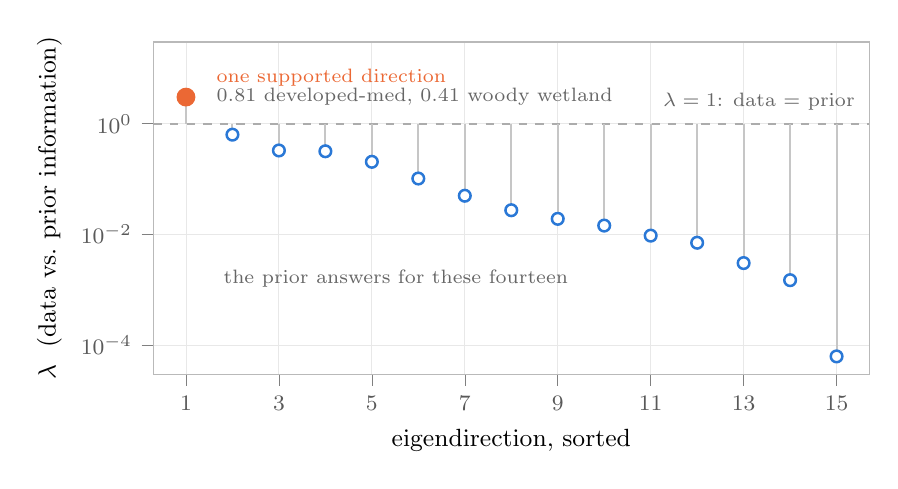
\begin{tikzpicture}
\begin{axis}[
  width=0.88\linewidth, height=5.8cm,
  xlabel={eigendirection, sorted},
  ylabel={$\lambda$ \ (data vs.\ prior information)},
  xmin=0.3, xmax=15.7,
  ymin=3e-5, ymax=30,
  ymode=log,
  xtick={1,3,5,7,9,11,13,15},
  tick align=outside, tick pos=left,
  axis line style={gray!55},
  tick label style={font=\footnotesize, color=black!65},
  label style={font=\small},
  grid=major, grid style={gray!18, line width=0.3pt},
  clip=false,
]

% the lambda = 1 threshold: data information equals prior information
\addplot[gray!65, line width=0.8pt, dashed, forget plot]
  coordinates {(0.3,1) (15.7,1)};
\node[font=\scriptsize, color=black!60, anchor=south east]
  at (axis cs:15.6,1.15) {$\lambda = 1$: data $=$ prior};

% stems
\addplot[ycomb, gray!45, line width=0.7pt, forget plot]
  coordinates {(1,3.033) (2,0.6353) (3,0.3292) (4,0.3183) (5,0.2055)
               (6,0.1025) (7,0.05008) (8,0.02742) (9,0.01917) (10,0.01448)
               (11,0.00953) (12,0.007093) (13,0.003043) (14,0.001495)
               (15,0.00006272)};

% the fourteen the prior determines
\addplot[only marks, mark=*, mark size=2.1pt,
         color={rgb,255:red,42;green,120;blue,214},
         mark options={fill=white, line width=0.9pt}, forget plot]
  coordinates {(2,0.6353) (3,0.3292) (4,0.3183) (5,0.2055)
               (6,0.1025) (7,0.05008) (8,0.02742) (9,0.01917) (10,0.01448)
               (11,0.00953) (12,0.007093) (13,0.003043) (14,0.001495)
               (15,0.00006272)};

% the one the data determines
\addplot[only marks, mark=*, mark size=3.2pt,
         color={rgb,255:red,235;green,104;blue,52},
         mark options={fill={rgb,255:red,235;green,104;blue,52}}, forget plot]
  coordinates {(1,3.033)};

\node[font=\scriptsize, color={rgb,255:red,235;green,104;blue,52},
      anchor=west, align=left]
  at (axis cs:1.45,4.6) {one supported direction\\[-1pt]
                         \textcolor{black!60}{$0.81$ developed-med, $0.41$ woody wetland}};
\node[font=\scriptsize, color=black!60, anchor=west, align=left]
  at (axis cs:1.6,0.0016) {the prior answers for these fourteen};
\end{axis}
\end{tikzpicture}

\caption{Eigenvalues of the prior-preconditioned Gauss--Newton Hessian
over the fifteen land-cover classes, sorted. Above $\lambda = 1$ the
marks constrain a direction more than the prior does; below it the
prior sets the answer. One
direction clears the line, and the remaining fourteen fall away over three
decades --- so a fifteen-parameter calibration is fitting one parameter
and inheriting fourteen from its prior. The log axis is not cosmetic: on
a linear one the cliff, which is the result, would be invisible.}
\label{fig:spectrum}
\end{figure}

$\lambda = 2.78,\ 0.68,\ 0.61,\ 0.32,\ 0.23,\ 0.10, \dots$
(Figure~\ref{fig:spectrum}) --- a single
eigenvalue above unity, a spectral gap of $4.1$, and $2.20$ degrees of
freedom for signal in Rodgers' sense. \textbf{These 46 marks support
one roughness parameter} --- one combination of the fifteen class
values on which the data out-weighs the prior, and no second.

A shorter pilot of the same configuration ($7{,}200$ steps, two event
hours) gives $\lambda = 3.03,\ 0.64,\ \dots$: the same count, the same
three leading classes, and a slightly \emph{larger} leading
eigenvalue. We had expected the opposite, since a longer window lets
each peak integrate more trajectory, and the reason it does not is
worth stating. Over two event hours many marks have not crested, so
the pilot's ``peak'' is often a point on a rising limb, and a rising
limb responds to roughness more sharply than a crest does --- at a
true maximum the first-order response in time has vanished by
definition. The longer window measures the observable the calibration
actually uses, and it is marginally less informative, not more. Any
argument that a longer experiment buys identifiability has to come
from more marks crossing into the window, not from more trajectory per
mark.

The scans and the spectrum agree, and they are
independent: no optimizer, no line search, and no calibration enters
Eq.~\eqref{eq:gn}.

\paragraph{But the scan varied nearly the wrong direction.}
The leading mode, with components
$-0.64$ on developed-medium, $+0.59$ on woody wetland, $-0.36$ on
developed-low and $-0.23$ on pasture, is dominated by the
large-area classes. Its overlap with the uniform direction the
$\alpha$-scan varies --- equal weight per \emph{class} --- is $0.218$,
which for fifteen classes is indistinguishable from random ($0.258$).
Its overlap with the same physical change weighted per \emph{cell} is
$0.699$. So the informative mode is the domain-scale conveyance mode we
claimed, but area-weighted; the $\alpha$-scan probes it only obliquely.
That is why the class calibration beats uniform scaling by $0.078$\,m
(Table~\ref{tab:ladder}): it is not that fifteen parameters beat one, it
is that the scan's one parameter was the wrong one.

\paragraph{What the calibration actually did.}
Projecting the calibrated displacement onto the eigenbasis is worth
reporting, and it cuts both ways. The calibrated field sits
\textbf{9.2 prior standard deviations} from the NLCD lookup, and of that
motion only $2.9\%$ lies in the single data-constrained direction;
$85.6\%$ lies in directions where data and prior are comparable and
$11.5\%$ where the prior alone determines the answer. Per class
(Table~\ref{tab:learned}) the marks shrink the prior uncertainty by
$30\%$ on developed-medium and $28\%$ on woody wetland, by
$11$--$20\%$ on three more, and by $5\%$ or less on the remaining ten.

The reassuring half is the null space. Two iterations in,
the optimizer had moved deciduous forest to $\alpha = 0.739$, mixed
forest to $1.096$ and cropland to $1.274$ --- three classes these marks
teach nothing about --- and by iteration nine accumulated curvature had
returned all three to within $10\%$ of the prior ($0.983$, $1.006$,
$1.098$). Those excursions were transients of an under-informed
quasi-Newton approximation rather than features of the minimizer: the
misfit gradient in uninformative directions is not zero, merely
uninformative, and given enough iterations the prior term dominates. A
calibration stopped early would have reported them as results, which is
an argument for running these problems to convergence even when the
objective has visibly flattened.

The unreassuring half is what survives. The residual $9.2\sigma$ is
concentrated in the two \emph{best}-informed classes, and both are
pressed against the edge of what the prior permits: developed-medium
sits at its $\alpha = 0.3$ lower bound for all nine iterations, and
woody wetland is driven to $\alpha = 0.355$, some $4.2\sigma$ from its
lookup value. So the displacement is not motion in directions the data
does not constrain. It lies in the one direction the data constrains,
toward roughness below what the published table and our stated prior
width jointly allow. Whether that value is admissible is not something
the optimizer can settle. We put the lookup's uncertainty at $30\%$ or
more, which admits it for the classes the marks constrain and, as the
spectrum shows, releases twelve that they do not.

\begin{table}
\centering\small
\begin{tabular}{@{}llrrr@{}}
\toprule
NLCD & class & prior $\sigma_n$ & posterior $\sigma_n$ & learned \\
\midrule
23 & developed medium & $0.015$ & $0.0105$ & $30\%$ \\
90 & woody wetland & $0.015$ & $0.0109$ & $28\%$ \\
81 & pasture & $0.015$ & $0.0121$ & $20\%$ \\
22 & developed low & $0.015$ & $0.0125$ & $17\%$ \\
21 & developed open & $0.015$ & $0.0133$ & $11\%$ \\
95, 24, 11, 31 & & $0.015$ & $0.014$--$0.015$ & $2$--$5\%$ \\
41, 43, 82, 42, 71, 52 & & $0.015$ & $0.015$ & $\le 1\%$ \\
\bottomrule
\end{tabular}
\caption{What the 46 marks constrain in each land-cover class, as the
fractional reduction from prior to posterior standard deviation, on the
production-window spectrum. Ten classes narrow by $5\%$ or less: any
value a calibration reports for them is the prior, not the data.}
\label{tab:learned}
\end{table}

\paragraph{A direct test: calibrate three classes instead of fifteen.}
Everything above is a statement about a matrix. It makes a prediction
an optimizer can falsify: if the marks really inform one direction,
then calibrating only the classes that carry that direction should
recover most of what all fifteen achieved --- and if it does not, the
information lives outside the leading eigenspace and the
one-parameter reading is too narrow. We ran it. Taking the three
classes with the largest components in the leading eigenvector
(developed-medium, woody wetland, developed-low), freezing the other
twelve at the prior, and calibrating from the NLCD lookup gives
$J = 682.1$ after four iterations --- the last two changing $J$ by
$0.02\%$ and $0.001\%$. Against the NLCD prior's $808.3$, three
parameters remove $126.1$ units where fifteen remove $150.9$:
\textbf{$84\%$ of the reduction from $20\%$ of the parameters.} The
twelve frozen classes were verified to sit bit-exactly at the prior in
the output, so the comparison is what it claims to be.

The prediction survives the change of metric, which is the sharper
test. Scored on peak-WSE MAE rather than on the objective it was fit
to, the three-parameter field reaches $0.6274$\,m against the NLCD
prior's $0.7188$ --- $85\%$ of the $0.107$\,m that fifteen parameters
achieve, and within a hair of the $84\%$ it recovered of the
objective. The two agree here, and they did not for the fifteen-class
field (Section~\ref{sec:calibrated}): a fit confined to the directions
the data constrains buys MAE at the same rate it buys objective, while
one free to move all fifteen does not. Three of these parameters also
beat the best physically defensible uniform field by $0.062$\,m,
so nearly all of what class-by-class calibration achieves over global
scaling is achieved by three classes.

Two details sharpen it further. The remaining $16\%$ is real, not
noise, and it decomposes exactly: the fifteen-parameter field pays
$8.8$ more units of prior penalty to buy $33.5$ more units of misfit
reduction.
So the twelve non-leading classes are not literally decoration --- in
aggregate they reach a few per cent of $J$ --- but they are not where
the information is. And the three parameters land where the
fifteen-parameter calibration put them: developed-low at
$\alpha = 1.626$ against $1.627$, developed-medium on its
$\alpha = 0.3$ bound in both. Two classes reproduced to three digits
from a different starting point and a different active set is the
behaviour of parameters the data actually determines. Woody wetland is
the exception and is instructive: alone it dives to $\alpha = 0.301$
where the full calibration left it at $0.355$, because with its
partners frozen it must supply their share of a change the marks
constrain only in combination --- equifinality, exactly where the
eigenvector says to expect it.

\paragraph{The same three classes under the fractional prior.}
The three-class run above used the absolute prior. Repeating it under
the fractional prior at $\sigma_\alpha = 0.30$, the width we assign to
the lookup, and at $0.50$ as a bracket above it, gives $0.6290$
and $0.6295$\,m (Table~\ref{tab:ladder}): $84\%$ and $83\%$ of the
fifteen-class error reduction, and $90\%$ and $94\%$ of its objective
reduction. The optimizer's path is short. At $\pm 30\%$ the first step
puts all three classes on a bound, exactly as it put seven of fifteen
there (Section~\ref{sec:calibration}), and two more iterations bring
developed-low back from $\alpha = 3$ to $2.34$; at $\pm 50\%$ the first
step lands on the corner of the box, the projected gradient there is
zero, and the run converges in one iteration. The Gaussian prior is not
what stops it: it contributes $15$ units to $J$ at $\pm 30\%$ and $10$
at $\pm 50\%$ against a misfit near $630$, so the bounds
$\alpha \in [0.3, 3]$ do the constraining.

Three things follow. Developed-medium reaches $\alpha = 0.3$ under
every prior and every active set we have run, and woody wetland does
whenever its two partners are frozen ($0.355$ and $0.64$ when they are
not --- the equifinality above), so in the three-class problem those
values are set by the data, and they are $n = 0.036$ and $0.029$,
below the lookup's $0.040$ for developed open land. Developed-low's
value is set by the prior: it moves from $1.63\times$ to $2.34\times$
to $3\times$ its lookup as the width opens while the MAE moves
$0.002$\,m, which is the flat direction the eigenvector predicted. The
three-parameter field therefore lies outside the prior as well. What
the spectrum selects is the calibration the marks can determine, and
what they determine is a roughness below the lookup's range at any
width we assign to it, which is evidence that the calibrated friction
is compensating for an error that lives elsewhere
(Section~\ref{sec:icauthority}).


\paragraph{Would more marks fix it?}
This is the natural objection --- 46 observations for 15 parameters
sounds like too few --- and Eq.~\eqref{eq:gn} answers it, because
$\lambda$ scales linearly in the number of comparable observations and
as $\sigma^{-2}$ in their quality (Table~\ref{tab:scaling}). The answer
is that more marks help, slowly, and that the supply is exhausted long
before the parameterization is justified. Going from the 46 marks of
this window to \emph{all} 71 the model can legitimately be scored
against supports two parameters. Every QC-passed mark in the
domain, over a window long enough to catch all of them, supports three.
Reaching five would take every Harvey mark that falls in the domain
including the $62\%$ that failed QC because they are channel surveys a
30\,m cell cannot represent. Fifteen would take of order $10^5$ marks.

\begin{table}
\centering\small
\begin{tabular}{@{}rrl@{}}
\toprule
Marks & Supported & That data set is \\
\midrule
46 & 1 & the cluster-A marks (this study) \\
71 & 2 & all admissible marks, 24-hour window \\
108 & 3 & every QC-passed mark, 72-hour window \\
324 & 5 & every Harvey mark in-domain, \emph{before} QC \\
$7\times10^5$ & 15 & --- \\
\bottomrule
\end{tabular}
\caption{How the supported-parameter count scales with survey size at
fixed quality ($\sigma = 0.15$\,m); a parameter is \emph{supported}
when the data narrows it more than the prior does ($\lambda > 1$). At fixed size, improving quality to
$\sigma = 0.10$\,m buys two more parameters (three in all) and $\sigma = 0.05$\,m --- better
than any high-water-mark survey achieves --- buys five. The table is a
benchmark, not a forecast: it assumes independent, equal-variance
residual errors and holds the measured per-mark sensitivity, the prior,
and the linearization fixed, so the longer-window rows describe mark
populations only, and a survey with correlated errors would enter
through $\Gamma^{1/2} S^\top C^{-1} S\, \Gamma^{1/2}$ rather than
through a count. That is the conservative reading
and, as it turns out, the correct one: we expected a longer window to
raise each mark's sensitivity and it does not (see text).}
\label{tab:scaling}
\end{table}

The conclusion is therefore not that Manning roughness is
unidentifiable. It is that \emph{surveyed peak water-surface elevations
at survey accuracy carry about two degrees of freedom of information
about distributed roughness in this basin}; that this can be computed
from sixteen forward runs before any optimizer is written; and that the
limitation is a property of the observing system rather than of the
method. A study that reported only its misfit reduction would have
concluded the opposite.

\section{Where else the error lives: the initial condition}
\label{sec:icauthority}

Roughness, calibrated as well as we can calibrate it, explains $15\%$
of this model's error against the marks. Something explains the other
$85\%$, and the candidates --- rainfall forcing, mesh elevation,
datum, representation error, the state the window starts from --- are
not all equally measurable. This section points the ceiling
measurement of Section~\ref{sec:authority} at the one candidate it can
probe with a single scan direction: the initial condition. The
initial state is also the input a variational initialization would
control, so the measurement doubles as a feasibility probe for
initial-state estimation with the same adjoint machinery, which the
conclusions take up.

Our window begins at event hour 29 from a checkpoint of the
72-hour forward, and the natural single direction to scan is the
amount of water that checkpoint holds. Scaling all three conserved variables by a common
factor $a$ changes antecedent storage while leaving every velocity
unchanged, since $u = (hu)/h$ is invariant. Each point is one forward
(Table~\ref{tab:ic}).

\begin{table}
\centering\small
\begin{tabular}{@{}lrrr@{}}
\toprule
IC scale $a$ & $J$ & MAE & $\Delta$MAE per $0.1$ \\
\midrule
$0.80$ & $6.652\times10^{2}$ & $0.6434$ & --- \\
$0.90$ & $7.284\times10^{2}$ & $0.6796$ & $+0.0362$ \\
$1.00$ (checkpoint) & $8.083\times10^{2}$ & $0.7188$ & $+0.0392$ \\
$1.10$ & $9.071\times10^{2}$ & $0.7610$ & $+0.0422$ \\
$1.20$ & $1.025\times10^{3}$ & $0.8174$ & $+0.0564$ \\
\bottomrule
\end{tabular}
\caption{Peak-WSE misfit against antecedent water storage. The response
is monotone over the whole range with no interior optimum, straight to
about $1\%$ between $a = 0.8$ and $1.1$ and convex above it: adding
water hurts at an accelerating rate. The model holds systematically too
much water at hour 29. No mark is dry at any point.}
\label{tab:ic}
\end{table}

Three things follow, and they matter more than the roughness result.

\textbf{The initial state has about four times the authority of
roughness} (Figure~\ref{fig:authority}). Per unit fractional change, $\mathrm{d}\,\mathrm{MAE}$ is
$0.392$ for the initial condition over its well-sampled range
($a \in [0.8, 1.1]$) against $0.098$ for a uniform roughness scale. Like for like at a $20\%$ perturbation: $0.075$\,m
versus $0.020$\,m. The plausibility runs the same way: a $20\%$ error
in water stored after a 29-hour spin-up under radar-derived rainfall
is within the uncertainty of that forcing~\cite{xu2025harvey}, while
Manning values at $30\%$ of the published table lie below the table's
own value for open land.

\textbf{The response has the opposite curvature to roughness's.}
$J(\alpha)$ for roughness is concave and saturating --- the knob runs
out --- consistent with a parameter acting indirectly through
path-integrated conveyance. $J(a)$ for the initial state is straight to
about $1\%$ between $a = 0.8$ and $1.1$ and \emph{convex} above,
steepening as water is added, and it does not turn over anywhere in the
range. Extending the scan below the table confirms it: at $a = 0.6$ ---
a $40\%$ reduction in antecedent water --- the MAE is still falling, to
$0.5818$\,m (Figure~\ref{fig:authority}). Neither the slope nor the
sign gives any indication of an
optimum near the checkpoint value. That is the signature of a
systematic bias rather than a poorly-tuned parameter: the model does not
hold slightly the wrong \emph{distribution} of water at hour 29, it
holds too much of it.

\textbf{It is a diagnosis, not a knob.} We are not proposing to
calibrate the initial condition against these marks. Over this window
the initial state carries $3$ unknowns on each of 2.93M cells against
46 peak observations, and everything Section~\ref{sec:authority}
establishes about identifiability applies with three more orders of
magnitude of freedom: such a calibration would fit the marks exactly
and mean nothing. What the scan does establish is the weaker
and more useful claim that the residual these marks measure lives substantially
in the water balance --- in the rainfall forcing or the antecedent state
--- rather than in the friction, which is where a roughness calibration
alone would have kept looking.

One caveat bounds all three. The checkpoint is a \emph{model} state, not
an observation, so it already contains accumulated forcing and elevation
error; the scan perturbs that state rather than an independent
measurement of it. A calibration of the initial condition would
therefore absorb such error rather than correct it, and could quietly
launder the downstream drainage defect of Section~\ref{sec:hwm} into a
``corrected'' initial state --- the same trap as scoring against the 37
marks the model cannot drain. Establishing whether a $20\%$
water-balance error at hour 29 is physically plausible is a question for
the forcing data, not for the optimizer. Our answer is that it is:
the antecedent state after a 29-hour spin-up under radar rainfall is
among the least certain inputs the model has, and an error of that
size in it is plausible. The uncertainty study of this event
in~\cite{xu2025harvey} finds precipitation and mesh resolution to dominate the simulated
inundation over the choice of outlet boundary condition~\cite{xu2025harvey},
which points the same way.

\section{Conclusions and outlook}

An exact, verified Jacobian turns out to be the single artifact from
which everything else follows cheaply: adjoint state and parameter
sensitivities, gradient-based calibration, and implicit stepping. The
capability is production-ready in the sense that matters for an
operational code --- behind a flag, FD-gated in CI, and with the
verification baseline (FD coloring) kept alive in the configuration
system.

The second artifact is a measurement rather than a capability, and it
is the one we would most like others to copy. Asking what fraction of
a model's error a parameter is \emph{able} to explain is cheap,
optimizer-independent, and it reframes what a calibration result
means. Here it bounded roughness at $4\%$ of the error within
defensible values and $11\%$ at the edge of plausibility; the
calibration then reached $15\%$, beating every global scaling and
confirming that letting roughness vary by class removes error a
single global factor cannot. What makes the measurement worth copying is not that
number but the two it led to. Pointed at the residual instead of the
parameter, the same machinery isolated a reach the model cannot drain;
pointed at the initial condition, it found more authority than
roughness has. A calibration study that had only reported its misfit
reduction would have found neither.

Next steps, in order. First, cross-validate the
calibration reported here --- nine quasi-Newton iterations stopped by
a wall-clock limit, with one class on a bound, is a fit, not
demonstrated skill --- and the held-out marks must come from within
the upstream band, because the middle band carries the drainage
defect. Second, calibrate the number of parameters
the observable supports rather than the number the land-cover map
offers; the spectrum of the prior-preconditioned Hessian would settle
that count directly, and at fifteen parameters it is a small dense
eigenproblem rather than a research project. Third, the water balance:
the initial-condition scan says the antecedent state carries more of
this residual than the friction does, which makes the forcing and the
initial condition --- not the roughness --- the next thing to
calibrate or diagnose, with the machinery applying unchanged and
$dJ/du_0$ already verified. Fourth, the conveyance and outlet
representation the drainage finding implicates. Finally, coupling the
gradient path to PyTorch through the existing
PETSc--PyTorch bridge for learned-physics and hybrid data-assimilation
experiments.

A closing note on cost. Checkpointing makes the long-window adjoint
memory-feasible, but at the 30\,m mesh's CFL-limited
$\Delta t = 0.25$\,s a full 36-hour Hurricane Harvey gradient still
costs several forward sweeps over half a million steps. The
affordable path stacks reductions that are all now in place. First,
fully implicit stepping at CFL-free time steps: backward Euler with
the assembled Jacobian carries the 30\,m, 2.93M-cell Harvey-region
mesh at $\Delta t = 1$\,s --- a step the differentiable explicit path
cannot take at any tested size (Section~\ref{sec:implicit}) --- with
Newton converging in about two iterations per step behind a
block-Jacobi-preconditioned Krylov solve at converged inner
tolerances; larger implicit steps are under investigation. Second, GPU execution of the entire gradient
pipeline: the right-hand side, the assembled Jacobian and its
transpose solves, the preconditioner setup, the parameter Jacobian,
the observation operator, and the revolve-checkpointed trajectory are
all device-resident. On four A100 GPUs, a forward-plus-adjoint
gradient of a one-simulated-hour window on that mesh (3{,}600
implicit steps, 400 in-memory checkpoints) takes about nine minutes,
and one TAO iteration of a dense-gauge twin calibration
(418{,}076 gauges, 39-step window) takes 1.7\,s --- roughly
$19\times$ one 64-core CPU node of the same system. Device and host
runs produce bitwise-identical trajectories under a common compiler
and gradients identical to every printed digit, so the
finite-difference gates of Table~\ref{tab:verification} carry over
unchanged. Third, land-cover-class parameterization (tens of TAO
evaluations instead of hundreds) and calibration windows placed on
the storm peak rather than the full event.

\section*{Code and data availability}
RDycore is open source at \url{https://github.com/RDycore/RDycore}; the
adjoint, Jacobian, implicit-stepping and calibration capability of this
paper is on the \texttt{adams/gpu-implicit} branch behind the
\texttt{numerics.jacobian} and \texttt{adjoint} configuration flags, and
the verification gates of Table~\ref{tab:verification} run in its
\texttt{ctest} suite. The exact revision, the campaign scripts, the
observation tables, and the per-mark peak dumps behind
Figures~\ref{fig:authority} and~\ref{fig:spectrum} will be archived on
Zenodo at submission \textbf{[DOI to be minted]}. Hurricane Harvey
high-water marks are the USGS Short-Term Network survey, retrieved
through the STN Flood Event Viewer API (\url{https://stn.wim.usgs.gov})
with the retrieval script and the filtered mark table in the archive;
stage records are USGS NWIS; rainfall is MRMS. \textbf{[Mesh, checkpoint, and rainfall archive: location to be
stated.]}

\bibliographystyle{unsrt}
\bibliography{manning-calibration}

\end{document}
